%!TEX root = ../thesis.tex
\chapter{A stochastic modelling approach to approximating fluid queues\label{sec: construction and modelling}}
In this chapter we develop a new discretisation of a fluid queue using a \emph{quasi-birth-and-death process with rational arrival process components} (QBD-RAP). In the following chapter, Chapter \ref{sec: conv} we prove the scheme converges weakly. To improve upon the discretisation of \cite{bo2013}, we argue that the shift from QBD to QBD-RAP is necessary. The QBD construction of \cite{bo2013} uses Erlang distributions to approximate the deterministic time that the fluid queue spends in an interval on the event that the phase is constant -- it is well known that the Erlang distribution is the distribution with the smallest variance in the class of Phase-type distributions of a given order \cite{as1987}, and in this sense is the best approximation to the determinstic behaviour we want to capture. 

By choosing a matrix-exponential distribution with sufficiently small variance, the QBD-RAP approximation can be made arbitrarily accurate. Due to its stochastic interpretation, the QBD-RAP discretisation ensures solutions are positive, even when discontinuities are present. Unlike slope limiters and post-hoc filtering, for the QBD-RAP the positivity preserving nature is a property of the discretised operator. 

The structure of this chapter is as follows. Section~\ref{sec: inspiration} motivates the idea using the QBD approximation of \cite{bo2014}. Sections \ref{sec: modelling} and \ref{sec: zero states} describe the modelling of certain events of the fluid queue with matrix exponential distributions to ultimately construct the behaviour of the QBD-RAP on the event that the QBD-RAP remains in a given level. Section~\ref{sec: dynamics} describes the dynamics of the construction and also constructs the level process of the QBD-RAP. Section~\ref{sec: boundary conditions} deals with modelling boundary behaviour. Section~\ref{sec: initial conditions} describes how to model initial conditions of the fluid queue. Section~\ref{sec: closing} introduces the concept of a \emph{closing operator} which maps the state space of the QBD-RAP to estimates of the density of the fluid queue. 


\section{Inspiration and motivation}\label{sec: inspiration}
The inspiration for our approach stems from the QBD-based discretisation of \cite{bo2013}. A QBD can be seen as a two dimensional CTMC, \(\{(L(t),\phi(t))\}_{t\geq 0}\), where \(\{L(t)\}\) is the discrete level, and \(\{\phi(t)\}\) is the phase. \cite{bo2013} discretise the state space of the fluid into small intervals of width \(\Delta\); denote these by \(\mathcal D_k=[k\Delta,(k+1)\Delta]\). Their approximation captures the dynamics of the phase process exactly, but discretises the level process of the fluid queue. Their approximation supposes that when \(L(t)=k,\,\phi(t)=i\), then \(X(t)\approx k\Delta,\,\phi(t)=i\). 

When in level \(k\) and phase \(i\), the approximation sees events at rate \(|T_{ii}| + |c_i|\Delta\). Upon an event, with probability \(T_{ij}/(|T_{ii}| + |c_i|\Delta)\) a change of phase from \(i\) to \(j\) is observed and the approximation remains in level \(k\); with probability \(|c_i|\Delta/(|T_{ii}| + |c_i|\Delta)\) a change of level occurs, to \(k+1\) if \(c_i>0\) and \(k-1\) if \(c_i<0\). The generator of their QBD approximation (for an unbounded fluid queue) is 
\[\bs B = \left[ \begin{array}{cccc} \ddots & \ddots & \ddots & \\ \bs B_{-1}(\Delta) & \bs B_0(\Delta) & \bs B_{+1}(\Delta) & \\  & \bs B_{-1}(\Delta) & \bs B_0(\Delta) & \bs B_{+1}(\Delta) \\ & \ddots & \ddots & \ddots \end{array} \right]\]
\begin{align}
\bs B_0 &= \bs T- \bs C\Delta, && \bs B_{-1} = \left[\begin{array}{ccc} \bs 0 & & \\ & \bs C_-\Delta & \\ & & \bs 0 \end{array}\right], && \bs B_{+1} = \left[\begin{array}{ccc} \bs C_+\Delta & & \\ & \bs 0 & \\ & & \bs 0\end{array}\right].
\end{align}
Bean and O'Reilly then take \(\Delta \to 0\) and show that the approximation converges weakly to the fluid queue. It seems that this is the best we can do if we want to keep the interpretation of the approximation as a QBD. We now elaborate on this point.

For a given \(\Delta\), the discretisation of Bean and O'Reilly supposes that, when the phase is \(i\) and on the event of no change of phase, the sojourn time in a given level has an exponential distribution with rate \(|c_i|\Delta\). However, the corresponding sojourn time of the fluid queue is deterministic: given \(X(t) = x \in\calD_k\), then \(\{X(t)\}\) will leave \(\calD_k\) in exactly \(((k+1)\Delta - x)/|c_i|\) units of time if \(c_i>0\), and \((x-k\Delta)/|c_i|\) units of time if \(c_i<0\), on the event that the phase does not change before this time. We can extend the QBD model of Bean and O'Reilly to model this determinism more accurately by supposing that the sojourn times in each interval have Erlang distributions (rather than exponential). However, we effectively realise the same QBD approximation as the original, but on a finer discretisation. For example, using Erlang distributions of order 2 we would get a generator of the QBD approximation
\[\bs B = \left[ \begin{array}{cccc} \ddots & \ddots & \ddots & \\ \bs B_{-1}(\Delta) & \bs B_0(\Delta) & \bs B_{+1}(\Delta) & \\  & \bs B_{-1}(\Delta) & \bs B_0(\Delta) & \bs B_{+1}(\Delta) \\ & \ddots & \ddots & \ddots \end{array} \right]\]
\begin{align}
\bs B_0 &= \bs T\otimes I_2 - \left[ \begin{array}{ccc} \left[\begin{array}{cc} -\Delta/2 & \Delta/2 \\ 0 & -\Delta/2 \end{array}\right] \otimes \bs C_+ & & \\ & \left[\begin{array}{cc} -\Delta/2 & 0 \\ \Delta/2 & -\Delta/2 \end{array}\right] \otimes C_- & \\ & & \bs 0 \end{array}\right], 
\end{align}
\begin{align}
\bs B_{-1} &= \left[\begin{array}{ccc} \bs 0 & & \\ & \bs C_-\otimes \left[\begin{array}{cc} 0 & \Delta/2 \\ 0 & 0 \end{array}\right] & \\ & & \bs 0 \end{array}\right],
&&\bs B_{+1} = \left[\begin{array}{ccc} \bs C_+\otimes \left[\begin{array}{cc} 0 & 0 \\ \Delta/2 & 0 \end{array}\right] & & \\ & \bs 0 & \\ & & \bs 0\end{array}\right].
\end{align}
But this is the same discretisation we would get if we were to use intervals of width \(\Delta/2\) in the QBD approximation of \cite{bo2013}, with the rows/columns reordered. Indeed, this appears to be the best we can do with a QBD approximation as the Erlang distribution is known to be the least variable Phase-type distribution for a given order \citep{as1987} and therefore gives the closest approximation to the deterministic behaviour we are trying to approximate. This necessitates the extension to QBD-RAPs, whereby we can find more concentrated distributions than any Phase-type and retain enough stochastic interpretation and matrix-analytic tools. 

Here, the construction of the approximating QBD-RAP is developed intuitively, from a stochastic modelling perspective. The key observation is that, given \(\{\varphi(t)\}\) is constant, then \(\{X(t)\}\) moves deterministically. Upon discretising the state space of the level process into intervals of width \(\Delta\), then, given \(X(t)\), the distribution of time it takes for \(\{X(t)\}\) to leave a given interval on the event that \(\{\varphi(t)\}\) remains in the same phase, is deterministic. We model this deterministic behaviour approximately by concentrated matrix exponential distributions (matrix exponential distributions with low-variance) \citep{ert2006,hstz2016,ert2006,hht2020,mt2021}. We construct a level process for the QBD-RAP and correspond it to a discretisation the level process of the fluid queue. This is similar to \cite{bo2013} where the level process of their QBD corresponds a discretisation of the fluid level. Unlike \cite{bo2013}, however, here we do not take \(\Delta \to 0\). Rather, we suppose that the variance of the concentrated matrix exponential distributions we use to approximate deterministic events gets small. % This necessarily means that the order of the matrix exponential increases. 

It turns out that the corresponding orbit process \(\{\bs A(t)\}\) can be seen to ``track", approximately, how far \(X(t)\) is from the left of a given interval when the phase is in \(\mathcal S_+\), or how far from the right of the interval \(X(t)\) is when the phase is in \(\mathcal S_-\). This leaves us with two problems. 1) on a transition from \(\mathcal S_+\) to \(\mathcal S_-\) or \(\mathcal S_-\) to \(\mathcal S_+\) how must \(\bs A(t)\) jump to retain this information about where \(X(t)\) is within a given interval. 2) how to use the orbit position at time \(t\), \(\bs A(t)\), to obtain an approximation for the density of \(X(t)\). Answers to both problems can be derived from the \emph{residual time} of a matrix exponential distribution. Let us now formalise these concepts some more. 

\section{Time to exit an interval}\label{sec: modelling}
Consider the partition of the state space of the level of a fluid queue, \([0,M]\) into \(K\) intervals of width \(\Delta = M/(K+1)\), specifically \(\mathcal D_{k,i} = [k\Delta,(k+1)\Delta)\) if \(i\in\mathcal S_+\) and \(\mathcal D_{k,i} = (k\Delta,(k+1)\Delta]\) if \(i\in\mathcal S_-\), \(k=0,\dots,K+1\). The distinction between \(\mathcal D_{k,i}\) for \(i\in\mathcal S_+\) and \(\calS_-\) is a technical one and will be discussed later. For now, one reason we might want to specify the discretisation in this way, is that it ensures the stochastic process 
\begin{align}
	\displaystyle \left\{\sum_{k\in\mathcal K}\sum_{i\in\calS} k1(X(t)\in\calD_{k,i})\right\}_{t\geq 0} \label{eqn: kfj}
\end{align}
is right-continuous with left limits (c\'adl\'ag). The expression (\ref{eqn: kfj}) is the discrete process of the fluid-queue which the level process of the QBD-RAP will approximate. Let \(y_k = k\Delta\), \(k=0,\dots,K+1\) and \(\calD_k = [y_k,y_{k+1}]\). We now look to model the behaviour of \(\{X(t)\}\) on an interval \(\calD_k\) over the time \([t,t+u]\) given information about the phase process over this time. 

\subsection{Modelling the residual time to exit on no change of phase} 
We first consider no change of phase in \([t,t+u]\). Suppose that \(\varphi(t)=i\in\mathcal S_+\) and \(X(t) = x\in\mathcal D_{k,i}\). Observe that on no change of phase, \(\varphi(t+s) = i\), \(s\in[0,u]\), and at time \(t+s\) the level of the fluid queue is given by \(X(t+s) = x+c_i s\), \(s\in[0,u]\). Further, for \(u>(y_{k+1}-x)/c_i\) the level process \(\{X(t)\}\) leaves the interval \(\mathcal D_{k,i}\) at exactly time \(t+(y_{k+1} - x)/c_i\). Similarly, for \(i\in\mathcal S_-\), \(\{X(t)\}\) leaves the interval \(\mathcal D_{k,i}\) at exactly time \(t+(x-y_k)/|c_i|\) on the event that there is no change of phase on \([t,t+u]\) for \(u>(x-y_k)/|c_i|\). 

To approximate the deterministic behaviour observed above, consider a matrix-exponential distribution \(Z\sim ME(\bs \alpha, \bs S, \bs s)\) with mean \(\Delta\) and low variance. As we shall see later, the assumption that \(Z\) has low variance will allow us to claim that \(Z\) can be used to approximate deterministic behaviour. Let \(Z_i\sim ME(\bs \alpha, \bs S_i, \bs s_i)\) where \(\bs S_i = |c_i|\bs S\), \(\bs s_i=-\bs S_i\bs e\), \(i\in\calS\). The random variable \(Z_i\) has mean \(\Delta/|c_i|\). 

Suppose first that \(X(t)=y_k\) and \(\varphi(t)=i\in\mathcal S_+\), so that \(X(t)\) will leave \(\mathcal D_{k,i}\) in exactly \(\Delta/|c_i|\) units of time on the event that the phase process of the QBD-RAP remains in \(i\) for at least this amount of time. A sensible approximation for this deterministic event is to choose the value of the orbit process at time \(t\) to be \(\bs \alpha\), \(\bs A(t)=\bs\alpha\). With this choice, the distribution of time until the next event of the QBD-RAP, on the event that the phase process remains constant will be the distribution of \(Z_i\). Observe, 
\begin{align*}
	\mathbb P(Z_i \in ((\Delta-\varepsilon)/|c_i|, (\Delta+\varepsilon)/|c_i|) ) 
	&= \mathbb P(Z\in (\Delta-\varepsilon, \Delta + \varepsilon))
%	\\&= \cfrac{\mathbb P(Z_i-u\in (\Delta/|c_i|-u-\varepsilon, \Delta/|c_i|-u + \varepsilon))}{\mathbb P(Z_i-u > 0)} 
%	\\&\geq \mathbb P(Z-u\in (\Delta-u-\varepsilon, \Delta-u + \varepsilon))
	\\&\geq 1-\cfrac{\var(Z)}{\varepsilon^2},
\end{align*}
since, by Chebyshev's inequality, \(\mathbb P(Z\in (\Delta-\varepsilon, \Delta + \varepsilon)) \geq 1- \cfrac{\var(Z)}{\varepsilon^2}\). Choosing \(\varepsilon = \var(Z)^{1/3}\), then 
\[\mathbb P(R_i(u) \in ((\Delta-\varepsilon)/|c_i|-u, (\Delta+\varepsilon)/|c_i|) )\geq 1-\var(Z)^{1/3} \approx 1, \]
when \(\var(Z)\) is small. Hence, when the variance of \(Z\) (equivalently \(Z_i\)) is low, then with high probability the time until the next event of the QBD-RAP, given the phase process remains constant will occur at approximately \(\Delta/|c_i|\). 

Now, let \(R_i(u)\) be the residual time, \(R_i(u) = (Z_i-u)1\{Z_i-u>0\}\), \(i\in\calS\). After \(u\in[0,\Delta/|c_i|)\) amount of time has elapsed, on the event that \(\varphi(t+s)=i\), for all \(s\in[0,u)\), then \(X(t+u) = y_k + c_i u\). If the phase remains \(i\) for a further \(\Delta/|c_i|-u\) amount of time, then \(\{X(t)\}\) will leave \(\calD_{k,i}\) at exactly this time. Also at time \(t+u\), given \(Z_i>u\), the distribution of the residual time, \(R_i(u)\), has density 
\[f_{R_i(u)}(r) = \cfrac{\bs\alpha e^{\bs S_i(u+ r) } \bs s_i}{\bs\alpha e^{\bs S_iu } \bs e} = \bs A(t+u) e^{\bs S_i r}  \bs s_i.\]
Here, the event \(Z_i>u\) approximates the event \(X(t+u)\in\calD_{k,i}\) and we want the residual time, \(R_i(u)\), to approximate the time until \(\{X(t)\}\) leaves \(\calD_{k,i}\). That is, we want \(R_i(u)\) to approximate a deterministic random variable at \(\Delta/|c_i| - u\). To this end, we observe that for \(\varepsilon>0\) and \(u<(\Delta-\varepsilon)/|c_i|\), then
\begin{align*}
	&\mathbb P(R_i(u) \in ((\Delta-\varepsilon)/|c_i|-u, (\Delta+\varepsilon)/|c_i|-u) ) 
	\\&= \mathbb P(Z_i\in ((\Delta-\varepsilon)/|c_i|, (\Delta+\varepsilon)/|c_i|) ) 
	\\&= \mathbb P(Z\in (\Delta-\varepsilon, \Delta + \varepsilon))
%	\\&= \cfrac{\mathbb P(Z_i-u\in (\Delta/|c_i|-u-\varepsilon, \Delta/|c_i|-u + \varepsilon))}{\mathbb P(Z_i-u > 0)} 
%	\\&\geq \mathbb P(Z-u\in (\Delta-u-\varepsilon, \Delta-u + \varepsilon))
	\\&\geq 1-\cfrac{\var(Z)}{\varepsilon^2}.
\end{align*}
Choosing \(\varepsilon = \var(Z)^{1/3}\), then 
\[\mathbb P(R_i(u) \in ((\Delta-\varepsilon)/|c_i|-u, (\Delta+\varepsilon)/|c_i|) )\geq 1-\var(Z)^{1/3} \approx 1, \]
when \(\var(Z)\) is small. 
That is, when the variance of \(Z\) (equivalently \(Z_i\)) is low, the residual time \(R_i(u)\) will be concentrated around \(\Delta/|c_i| - u\), as required. Figure \ref{fig:residual distributions} gives an example of a density function for a \(Z_i\) with mean \(\Delta=1\) and \(c_i=1\), as well as the density function of \(R_i(0.3)\) conditional on \(Z_i>0.3\) and \(R_i(0.6)\) conditional on \(Z_i>0.6\), for comparison. Observe that the density of the residual life \(R_i(0.3)\) conditional on \(Z_i>0.3\) is concentrated around \(\Delta-0.3 = 0.7\) and, similarly the density of the residual life \(R_i(0.6)\) conditional in \(Z_i>0.6\) is concentrated around \(\Delta-0.6 = 0.4\).

\begin{figure}
\centering
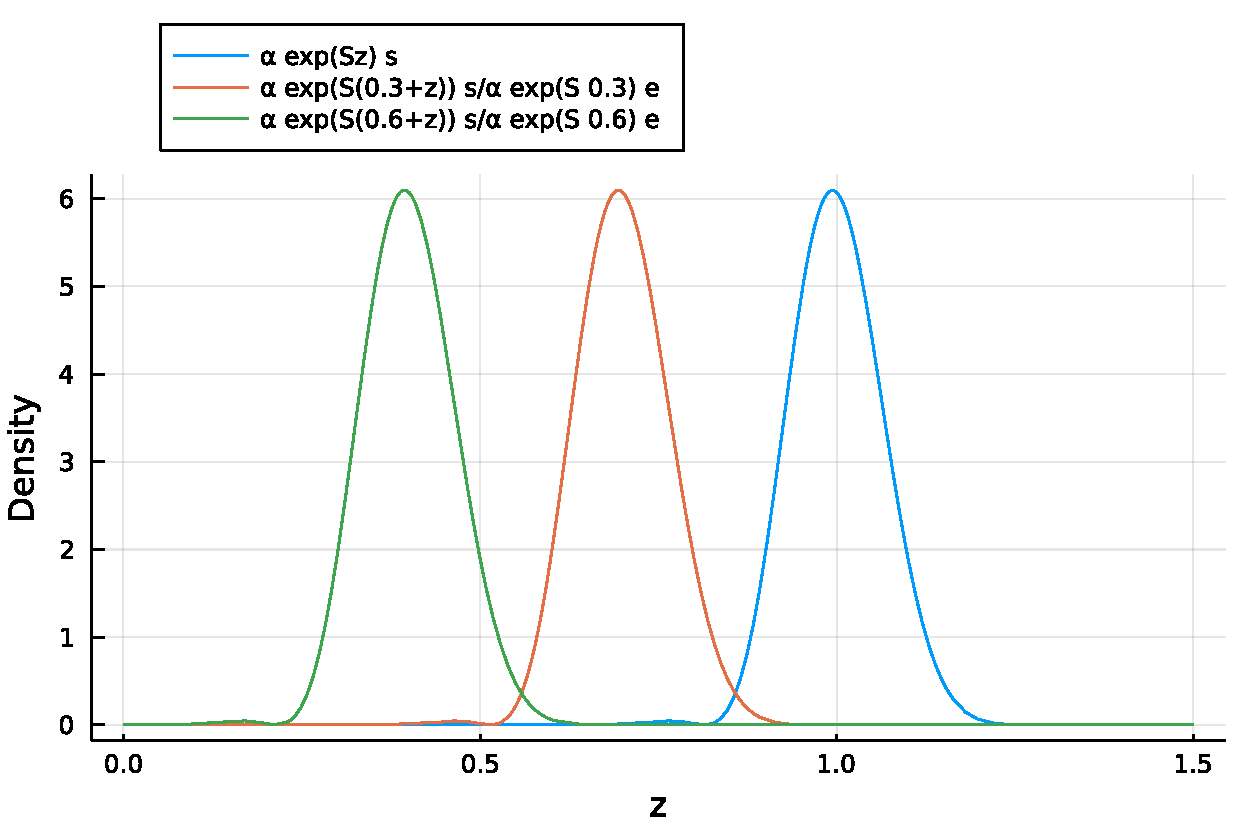
\includegraphics[width=\textwidth]{chapter2/figs/ME_residual_life_density.pdf}
\caption{The density function for a \emph{concentrated matrix exponential of order 21} from \citep{hht2020} (blue) and corresponding density functions of the residual lives, \(R_{0.3}\) (red), \(R_{0.6}\) (blue). Observe how the density function of the \(Z_i\) (blue) to approximate a point mass at \(\Delta=1\), while the density functions of \(R_{0.3}\) (red) and \(R_{0.6}\) (blue) approximate point masses at \(0.7\) and \(0.4\), respectively. }
\label{fig:residual distributions}
\end{figure}

For notational convenience, define the row-vector-valued function \(\bs k(t):\mathbb R\to \mathcal A\), 
\begin{equation}
	\bs k(t) = \cfrac{\bs \alpha e^{\bs S t}}{\bs \alpha e^{\bs S t}\bs e}, \label{eqn: orbit fun def}
\end{equation}
and the operator \(\bs K(t): \mathcal A\to \mathbb R\), \(t\geq 0\), 
\begin{equation}
	\bs a \bs K(t) = \cfrac{\bs a e^{\bs S t}}{\bs a e^{\bs S t}\bs e}, \label{eqn: operator fun def}
\end{equation}
for any \(a\in\mathcal A\). 

We interpret the position of the orbit \(\bs A(t+u) = \bs k(|c_i|u)\) as corresponding to the fact that \(X(t+u)\) is \(|c_i|u\) units from the left-hand boundary of the interval \(\calD_{k,i}\). This gives a heuristic argument as to how we can model the sojourn times in a given interval \(\mathcal D_{k,i}\) on the event that the phase does not change. 

We can apply analogous arguments to heuristically develop a model for the sojourn time of the fluid queue in an interval, \(\calD_{k,i}\), \(i\in\calS_-\), on the event that the phase does not change, given the fluid is \(X(t)=y_{k+1}\). For \(i\in\calS_-\), the orbit position \(\bs A(t+u) = \bs k(|c_i|u)\) is interpreted as corresponding to \(X(t)\) being \(|c_i|u\) units from the right-hand boundary of the interval \(\calD_{k,i}\), \(y_{k+1}\). 

\subsection{On a change of phase from \(i\in\calS_+\) to \(j\in\calS_+\)} 
%Let \(Z_j\sim ME(\bs\alpha,\bs S_j)\) be a matrix exponential random variable with mean \(\Delta/|c_j|\) and let \(R_j(u)\) be the residual time \(R_j(u) = Z_j-u \mid\{Z_j-u>0\}\). %At time \(t+u\) the value of the orbit is \(\bs A(t+u) =  \cfrac{\bs\alpha e^{\bs S_iu } }{\bs\alpha e^{\bs S_iu } \bs e}\), which can be equivalently written as \(\bs A(t+u) =  \cfrac{\bs\alpha e^{\bs S_ju/|c_i| } }{\bs\alpha e^{\bs S_ju/|c_i| } \bs e}\).

Let \(E\) be the event that, at time \(t\) the orbit of the QBD-RAP is \(\bs A(t) = \bs \alpha\), the phase process is \(\varphi(t) = i\in\calS_+\), and there are no events of the QBD-RAP before time \(t+u\). On the event \(E\) the orbit position at time \(t+u\) will be 
\begin{align}
	\bs A(t+u) = \bs k(|c_i|u) = \cfrac{\bs \alpha e^{\bs S_i u}}{\bs \alpha e^{\bs S_i u}\bs e}.\label{eqn: orbit i}
\end{align}
Correspondingly, on the event that at time \(t\) the level process of the fluid queue is \(X(t)=y_{k}\), the phase is \(\varphi(t)=i\) and there are no change of phase by time \(t+u\), then \(X(t+u)=y_{k}+c_iu\). That is, \(X(t+u)\) is \(c_iu\) units from the left-hand edge of \(\calD_k\). 

If, at time \(t+u\) there is a change of phase from \(i\in\calS_+\) to \(j\in\calS_+\), then we need to map the orbit position \(\bs A(t+u^-) = \bs k(|c_i|u)\) to an orbit position which corresponds to the being \(c_iu\) units from the left-hand edge of \(\calD_k\) in phase \(j\). Call this mapping \(\bs D(i,j)(\cdot)\). As noted in Section \ref{sec: qbd-rap}, the mapping must be linear, 
\(\bs D(i,j)(\bs a) = \bs a \bs D(i,j),\, \bs a \in\mathcal A,\)
for some matrix \(\bs D(i,j)\). The matrix \(\bs D(i,j)\) is a modelling choice. 

So that the process is a QBD-RAP, the matrix \(\bs D(i,j)\) must have the property that, for any \(\bs a\in\mathcal A\), \((\bs a\bs D(i,j), \bs S)\) is a representation of a matrix exponential distribution. We would also like the matrix \(\bs D(i,j)\) to have the property \(\bs D(i,j) \bs e = \bs e\) as this will mean that the rate at which a change of phase from \(i\) to \(j\) of the QBD-RAP occurs proportional to 
\[\bs A(t+u) \bs D(i,j)\bs e = 1,\]
which is constant and therefore the distribution of time until a change from phase \(i\) to \(j\) is exponential. We can use this to show, for certain models, the distribution of the phase process of the fluid queue and the distribution of the phase process of the QBD-RAP share the same distribution.

An orbit position which corresponds to the level process of the QBD-RAP beign \(c_iu\) units to the right of \(y_k\) in phase \(j\in\calS_+\) is 
\[\bs A(t+u) = \cfrac{\bs \alpha e^{\bs S_j (|c_i|u/|c_j|)}}{\bs \alpha e^{\bs S_j (|c_i|u/|c_j|) u}\bs e}.\] 
To see this, consider the event that at time \(t\) the orbit process of the QBD-RAP is \(\bs A(t) = \bs \alpha\), the phase process is \(\varphi(t) = j\in\calS_+\), and there are no events of the QBD-RAP before time \(t+|c_i|u/|c_j|\). On this event, the orbit position at time \(t+u\) will be 
\[\displaystyle \bs A(t+u) = \cfrac{\bs \alpha e^{\bs S_j (|c_i|u)/|c_j|}}{\bs \alpha e^{\bs S_j (|c_i|u/|c_j|) u}\bs e}.\] 
Correspondingly, on the event that at time \(t\) the level process of the fluid queue is \(X(t)=y_{k}\), the phase is \(\varphi(t)=j\) and there are no change of phase by time \(t+|c_i|u/|c_j|\), then \(X(t+u)=y_{k}+c_j|c_i|u/|c_j| = y_k+c_iu\). That is, \(X(t+u)\) is \(c_iu\) units from the left-hand edge of \(\calD_k\). 

Now, observe 
\[\cfrac{\bs \alpha e^{\bs S_j (|c_i|u/|c_j|)}}{\bs \alpha e^{\bs S_j (|c_i|u/|c_j|) u}\bs e} = \cfrac{\bs \alpha e^{\bs S_iu}}{\bs \alpha e^{\bs S_i u}\bs e} = \bs k(|c_i|u),\] 
which is exactly (\ref{eqn: orbit i}), the orbit position on the event \(E\). Hence, it is sensible to choose \(\bs D(i,j)=\bs I\). 

% Consider the residual time \(R_j(|c_i|u/|c_j|)\), which is the distribution of time until \(Z_j-|c_i|u/|c_j|\) occurs, on the event \(Z_j>|c_i|u/|c_j|\). The initial vector associated with the residual time \(R_j(|c_i|u/|c_j|)\) is \(\cfrac{\bs \alpha e^{\bs S_j |c_i|u/|c_j| } }{\bs \alpha e^{\bs S_j |c_i|u/|c_j|} \bs e }\). This is the initial vector which is obtained if at time \(t\) the phase is \(\varphi(t)=j\) and the orbit is \(\bs A(t)=\bs \alpha,\) so that the QBD-RAP has just entered level \(k\), and there is no change of phase by time \(|c_i|u/|c_j|\). Above, we argued that the vector \(\cfrac{\bs \alpha e^{\bs S_j |c_i|u/|c_j| } }{\bs \alpha e^{\bs S_j |c_i|u/|c_j|} \bs e }\) can be seen to correspond to the event that \(X(t+u)\) is \(|c_j|\left(|c_i|u/|c_j|\right) = |c_i|u\) units greater than \(y_k\). 
% %We argued earlier that the vector \(\cfrac{\bs \alpha e^{\bs S_j |c_i|u/|c_j| } }{\bs \alpha e^{\bs S_j |c_i|u/|c_j|} \bs e }\) is the position of the orbit on the event that at time \(t\) there is a change of level so that \(\bs A(t)=\bs \alpha\), and the phase is \(\varphi(t)=j\), followed by no change of phase by time \(t+|c_i|u/|c_j|\). The analogous event of the fluid queue is that at time \(t\) the phase is \(\varphi(t)=j\), the fluid level is \(X(t)=y_k\), so that the fluid level has just entered an interval \(\calD_k\) at time \(t\), and there is no change of phase by time \(t+|c_i|u/|c_j|\), in which case the fluid level will be \(X(t+|c_i|u/|c_j|)=y_\ell + |c_j|\left(|c_i|u/|c_j|\right)=y_\ell + |c_i|u\). Therefore, we claim that the vector \(\cfrac{\bs \alpha e^{\bs S_j |c_i|u/|c_j| } }{\bs \alpha e^{\bs S_j |c_i|u/|c_j|} \bs e }\) is the correct position of the orbit to approximate the fact that \(\{X(t)\}\) is \(|c_i|u\) units to the right of the point \(y_k\).

% Notice that we can re-write the vector 
% \(\cfrac{\bs \alpha e^{\bs S_j |c_i|u/|c_j| } }{\bs \alpha e^{\bs S_j |c_i|u/|c_j|} \bs e }\) as \(\cfrac{\bs \alpha e^{\bs S_iu } }{\bs \alpha e^{\bs S_iu} \bs e }\). This is the orbit position on the event that at time \(t\) there is a change of level, so that \(\bs A(t)=\bs \alpha\), and the phase is \(\varphi(t)=i\), followed by no change of phase by time \(t+u\). We have argued that this is the orbit position which approximates the fact that \(\{X(t)\}\) is \(|c_i|u\) units greater than \(y_k\). 

% Therefore, at time \(t+u\), if there is a change of phase from \(i\in\calS_+\) to \(j\in\calS_+\) then the orbit position should not change as in both cases the orbit position \(\cfrac{\bs \alpha e^{\bs S_j |c_i|u/|c_j| } }{\bs \alpha e^{\bs S_j |c_i|u/|c_j|} \bs e }\) corresponds to an approximation to \(X(t)\) being \(|c_i|u\) units greater than \(y_k\). 

%Therefore, suppose that at time \(t\), \(X(t)=y_k\), and that at time \(t+u\), \(u\in[0,\Delta/|c_i|)\), before \(\{X(t)\}\) exits the band \(\calD_{k}\), there is a change of phase from \(i\in\calS_+\) to \(j\in\calS_+\). At time \(t+u\) the position of the fluid level is \(X(t+u) = y_k+c_iu\), which is \(|c_i|u\) units to the right of \(y_k\) and \(\Delta-c_iu\) to the left of \(y_{k+1}\), the right-hand boundary of \(\calD_{k,i}\). The residual time until the level of the fluid queue leaves \(\calD_{k,j}\), on the event that it remains in phase \(j\) until this time, is \((\Delta - |c_i|u)/|c_j|\). 

Moreover, the residual time \(R_j(|c_i|u/|c_j|)\) has density 
\[f_{R_j(|c_i|u/|c_j|)}(r) = \cfrac{\bs\alpha e^{\bs S_iu } }{\bs\alpha e^{\bs S_iu } \bs e}e^{\bs S_j r}\bs s_j,\]
%and corresponds to an orbit position of \(\bs A(t+u) = \cfrac{\bs\alpha e^{\bs S_iu } }{\bs\alpha e^{\bs S_iu } \bs e}\). 
and 
\begin{align}
	&\mathbb P(R_j(|c_i|u/|c_j|) \in ((\Delta-|c_i|u-\varepsilon)/|c_j|, (\Delta-|c_i|u + \varepsilon)/|c_j| )) \nonumber
	\\&=\mathbb P(Z_j\in ((\Delta-\varepsilon)/|c_j|, (\Delta + \varepsilon)/|c_j|)) 
	\\&=\mathbb P(Z\in (\Delta-\varepsilon ,  \Delta + \varepsilon )) 
	% \\&=  \mathbb P(Z_j\in (\Delta/|c_j|-\varepsilon, \Delta/|c_j| + \varepsilon)) 
%	\\&= \cfrac{\mathbb P(Z_i-u\in (\Delta/|c_i|-u-\varepsilon, \Delta/|c_i|-u + \varepsilon))}{\mathbb P(Z_i-u > 0)} 
%	\\&\geq \mathbb P(Z-u\in (\Delta-u-\varepsilon, \Delta-u + \varepsilon))
%	\\&\geq \cfrac{1-\cfrac{\var(Z_j)}{\varepsilon^2}}{1} 
	\\&\geq 1-\var(Z)^{1/3} \approx 1.
\end{align}
Hence, when the variance of \(Z\) is low, the residual time, \(R_j(|c_i|u/|c_j|)\), is concentrated around \((\Delta - |c_i|u)/|c_j|\), as required. 

% Therefore, in our model, upon the event of a change from \(i\in\calS_+\) to \(j\in\calS_+\) at time \(t+u\) the orbit should be \(\bs A(t+u) = \cfrac{\bs\alpha e^{\bs S_iu } }{\bs\alpha e^{\bs S_iu } \bs e}\). That is, the initial condition for the next segment of the orbit process is just the current orbit position and the orbit should start to evolve according to the matrix \(\bs S_j\).

Analogous arguments suggest that the same applies for changes of phase from \(i\in\calS_-\) to \(j\in\calS_-\). 

\subsection{On a change of phase from \(i\in\calS_+\) to \(j\in\calS_-\)} 
Now suppose \(X(t)=y_k\), \(\varphi(t)=i\in\calS_+\), and the phase remains in state \(i\) until there is a change of phase from \(i\in\calS_+\) to \(j\in\calS_-\) at time \(t+u\), \(u\in[0,\Delta/|c_i|)\). %We have reasoned, intuitively, that, for \(i\in\calS_+\) and for \(x=|c_i|u\in[0,\Delta)\), the orbit position \(\bs k(x)\) corresponds to the fluid level position \(X(t) = y_k+x\), that is \(x\) units greater than \(y_k\).  
As before, we need to find a matrix \(\bs D(i,j)\) to map the orbit position on the event \(E\) when there is a change of phase from \(i\in\calS_+\) to \(j\in\calS_-\) at time \(t+u\), from \[\bs A(t+u^-) = \bs k(|c_i|u^-),\] 
to 
\[\bs A(t+u) = \cfrac{\bs k(u^-)\bs D(i,j)}{\bs k(u^-)\bs D(i,j)\bs e}=\cfrac{\bs\alpha e^{\bs S_iu} \bs D(i,j)}{\bs\alpha e^{\bs S_iu}\bs D(i,j)\bs e}\]
in such a way that the orbit position after the jump corresponds, in some way, to the fluid level being a distance of \(|c_i|u\) from \(y_k\) in phase \(j\). 

Again, the matrix \(\bs D(i,j)\) is a modelling choice. We first discuss how we might choose the matrix \(\bs D(i,j)\) for when the matrix-exponential \(Z\) is a phase-type distribution. 

\paragraph{The Phase-type case}
If \(Z\sim ME(\bs \alpha, \bs S)\) is chosen to be a phase-type distribution then \(Z\) has the interpretation as the distribution of time until absorption of a finite-state continuous-time Markov chain with transient states \(\{1,\dots,p\}\) and a single absrobing state. The sub-generator matrix describing the dynamics of the Markov chain on transient states is \(\bs S\), and \(\bs \alpha\) is an initial probability distribution over the transient states. Let \(\{J(t)\}\) be the Markov chain associated with the phase-type distribution. 

In the discussions above, we have relied on the relationship between the event \(E\) and the orbit position \(\displaystyle \bs k(|c_i|u)\). The relationship allows us to associate this orbit position with the level of the fluid queue. For phase-type distributions the vector \(\bs k(|c_i|u)\) is the vector of posterior probabilities \(\left[\mathbb P(J(u)=k \mid E)\right]_{k\in\{1,...,p\}}\). We can use this vector of posterior probabilities in the same way as we do for matrix-exponential distributions and QBD-RAPs. However, the orbit interpretation forgoes the presence of the phase process \(\{J(t)\}\). Here, we will use the phase process \(\{J(t)\}\) to derive a choice of \(\bs D(i,j)\). 

Recall the position of the orbit process can be used to determine the residual time. This idea can be replicated when we are given the phase of the phase-type rather than the value of the orbit process. Given the phase of the phase-type distribution is \(k\in\{1,...,p\}\), the distribution of the residual time is 
\[\mathbb P(R_i\leq r \mid \mbox{phase}=k)=1-\bs e_k e^{\bs S_i r}\bs e.\]
Notice that this is independent of the time since the phase-type distribution was initialised. We call the time since the phase-type distribution was initialised the \emph{age}. As noted by \cite{hmp2017}, the distribution of the age given the phase of the phase-type is \(k\in\{1,...,p\}\) depends on the sampling scheme which determines the observation time. Here, on the event that at time \(t\) the phase of the QBD-RAP is \(i\), a change of phase occurs after an exponential amount of time with rate \(-T_{ii}\). Proposition 4.1, \cite{hmp2017} states that the distribution function of the age, given the phase of the phase-type is \(k\) and the process is observed after an exponential time with rate \(-T_{ii}\) is 
\[\mathbb P(\mbox{age}\leq u \mid \mbox{phase}=k )=1-\cfrac{\bs \alpha e^{(\bs S_i + T_{ii}\bs I)u}(-(\bs S_i+ T_{ii}\bs I))^{-1}\bs e_k}{\bs \alpha (-(\bs S_i+ T_{ii}\bs I))^{-1}\bs e_k}.\]
Let \(\widehat{ \bs S}_i(T_{ii}) = diag(\bs \nu)^{-1}\bs S_i'diag(\bs \nu)\), where \(\bs \nu = \bs\alpha(-(\bs S_i+ T_{ii}\bs I))^{-1}/(\bs\alpha(-(\bs S_i+ T_{ii}\bs I))^{-1}\bs e)\). Algebraic manipulations show
\begin{align}
	1-\cfrac{\bs \alpha e^{(\bs S_i + T_{ii}\bs I)u}(-(\bs S_i+ T_{ii}\bs I))^{-1}\bs e_k}{\bs \alpha (-(\bs S_i+ T_{ii}\bs I))^{-1}\bs e_k}
	= 1-\bs e_k' e^{(\widehat{\bs S}_i(T_{ii}) + T_{ii}\bs I)u} \bs e,\label{eqn: skgj}
\end{align}
which is of Phase-type. 

Recall that in the matrix-exponential case we associated the value of the orbit process \(\bs k(|c_i|u)\) with being \(|c_i|u\) units to the right of \(y_{k}\). In contrast, for the phase-type case if we use the phase process \(\{J(t)\}\) to inform our modelling of the fluid queue (as opposed to the value of the orbit process), then we associate phase \(k\in\{1,...,p\}\) of \(\{J(t)\}\) with being a \emph{random} distance to the right of \(y_k\) where this distance has distribution 
\begin{align}
	1-\bs e_k' e^{(\widehat{\bs S}_i(T_{ii}) + T_{ii}\bs I)u} \bs e.\label{eqn: skgj2}
\end{align}
Therefore, on the event \(E\), upon a change from of phase of the QBD-RAP from \(i\in\calS_+\) to \(j\in\calS_-\) at time \(t+u\), it seems reasonable to want the distribution of time until the next event of the QBD-RAP to be
\begin{align}
	1-\bs e_k' e^{(\widehat{\bs S}_i(T_{ii}) + T_{ii}\bs I)|c_j|u/|c_i| + T_{jj}Iu} \bs e.\label{eqn: skgj3}
\end{align}
The factor \(|c_j|u/|c_i|\) arises as a conversion between the speed at which the fluid level moves in phase \(j\) compared to phase \(i\). The rate \(T_{jj}\) in the exponent is the rate at which the next change of phase occurs. 

While this does achieve what we want, it is not quite satisfactory for the purpose of our approximation scheme due to dependence on the sample path of \(\{\varphi(t)\}\). Specifically, the evolution of the QBD-RAP from time \(t+u\) until the next event depends on the phase immediately before the change of phase at time \(t+u\), \(\varphi(t+u^-)=i\). This increases the size of the approximating QBD-RAP as we need a separate model for each \(\varphi(t+u^-)\in\calS_+\). Furthermore, we have not yet considered how to model any further changes from \(\calS_-\) to \(\calS_+\) or beyond, which further complicates matters. 

A solution is to suppose that, rather than observing the phase-type random variable at an exponential time with rate \(-T_{ii}\), we instead observe the process uniformly randomly on the lifetime of length \(Z_i\). Let \(\bs \Pi = diag\left(\bs \pi \right)\), where \(\vligne{\pi_k}_{k\in\{1,\dots,p\}}=:\bs \pi=\bs \alpha (-\bs{S})^{-1}/m\) and \(m=\bs \alpha (-\bs{S})^{-1}\bs e\). There is a time-reverse representation of a Phase-type distribution given by \((\widetilde{\bs \alpha}, \widetilde{\bs S}, \widetilde{\bs s})\), where \(\widetilde{\bs \alpha} = m\bs s' \bs \Pi \), \(\widetilde{\bs S} = \bs\Pi^{-1}\bs S'\bs \Pi\) and \(\widetilde{\bs s} = \bs \Pi^{-1}\bs \alpha'/m\) \cite[Page 91]{a2008}. In the case where the phase is observed randomly on the lifetime of \(Z_i\), the distribution function of the age, given the phase is \(k\) is \cite[Lemma 3.1]{hmp2017}
\begin{align}\mathbb P(\mbox{age}\leq u \mid \mbox{phase}=k) = 1-\cfrac{\bs \alpha e^{\bs S_iu}(-\bs S_i)^{-1}\bs e_k}{\bs \alpha (-\bs S_i)^{-1}\bs e_k} = 1- \bs e_k e^{\widetilde{ \bs S}_iu}\bs e.\label{eqn:ksda2}\end{align}
With this interpretation, we may associate phase \(k\in\{1,...,p\}\) of \(\{J(t)\}\) with being a \emph{random} distance, with distribution (\ref{eqn:ksda2}), to the right of \(y_k\).

Therefore, on the event \(E\) and on a change of phase from \(i\in\calS_+\) to \(j\in\calS_-\) at time \(t+u\), a reasonable model for the time until the next event of the QBD-RAP has distribution 
\begin{align}
	1- \bs e_k e^{\widetilde{ \bs S}_iu|c_j|/|c_i| + T_{jj}\bs Iu}\bs e = 1- \bs e_k e^{\widetilde{ \bs S}_ju+ T_{jj}\bs Iu}\bs e.\label{eqn:ksda3}
\end{align}
This suggests that, at a jump from \(\calS_+\) to \(\calS_-\), the state of \(\{J(t)\}\) does not change, but begins to evolve according to the time-reverse generator at an appropriate speed. Since the time-reverse of \(\widetilde{\bs S}\) is \(\bs S\), then upon a jump back to \(\calS_+\) from \(\calS_-\), the phase of the phase-type random variable remains \(k\) but begins to evolve according to \(\calS\). This suggests that we use the representation \((\bs \alpha, \bs S)\) when in phases in \(\calS_+\), and use the time-reverse representation \((\widetilde{\bs \alpha}, \widetilde{\bs S})\) when in phases in \(\calS_-\). The matrices \(\bs D(i,j)=\bs I\) for all \(i,j\in\calS\). 

With this construction, and choosing \(Z\sim Erlang(p,\Delta/p)\), we recover the discretisation of \cite{bo2013} with discretisation parameter \(\Delta/p\).

% Let \(\bs \Pi = diag\left(\bs \pi \right)\), where \(\vligne{\pi_k}_{k\in\{1,\dots,p\}}=:\bs \pi=\bs \alpha (-\bs{S})^{-1}/m\) and \(m=\bs \alpha (-\bs{S})^{-1}\bs e\). There is a time-reverse representation of a Phase-type distribution given by \((\widetilde{\bs \alpha}, \widetilde{\bs S}, \widetilde{\bs s})\), where \(\widetilde{\bs \alpha} = m\bs s' \bs \Pi \), \(\widetilde{\bs S} = \bs\Pi^{-1}\bs S'\bs \Pi\) and \(\widetilde{\bs s} = \bs \Pi^{-1}\bs \alpha'/m\) \cite[Page 91]{a2008}.

% Rather than use the residual time \(R_i(u)\) to estimate how far \(X(t)\) is from the edge of an interval, we can use the information contained in \(J(t+u)\). Suppose there is a change of phase of the fluid queue from \(i\in\calS_+\) to \(j\in\calS_-\) at time \(t+u\) at which time \(J(t+u)=k\). At a random time before \(t+u\) the Phase-type random variable was initialised. Let \(C_{t+u}\) be the \emph{age} of the Phase-type distribution at time \(t+u\), that is, the time since the Phase-type random variable was initialised. Suppose that \(\varphi(v)=i\), \(v\in [t+u-C_{t+u}, t+u)\), that is, there has been no change of phase of the fluid queue during the current life of the Phase-type random variable. Given \(J(t+u)=k\), we wish to construct an approximation to the distribution of \(C_{t+u}\). 

% According to \cite{hmp2017}, the distribution of \(C_{t+u}\) depends on the method of observation. Here, the Phase-type distribution is observed after an exponential time with rate \(-T_{ii}\). Proposition 4.1, \cite{hmp2017} states that the cumulative distribution function (CDF) of \(C_{t+u}\), given \(J(t+u)=k\) and the process is observed after an exponential time with rate \(-T_{ii}\) is 
% \[\mathbb P(C_{t+u}\leq a )=1-\cfrac{\bs \alpha e^{(\bs S_i + T_{ii}\bs I)a}(-(\bs S_i+ T_{ii}\bs I))^{-1}\bs e_k}{\bs \alpha (-(\bs S_i+ T_{ii}\bs I))^{-1}\bs e_k}.\]
% Let \(\widehat{ \bs S}_i(T_{ii}) = diag(\bs \nu)^{-1}\bs S_i'diag(\bs \nu)\), where \(\bs \nu = \bs\alpha(-(\bs S_i+ T_{ii}\bs I))^{-1}/(\bs\alpha(-(\bs S_i+ T_{ii}\bs I))^{-1}\bs e)\). Algebraic manipulations show
% \begin{align}
% 	1-\cfrac{\bs \alpha e^{(\bs S_i + T_{ii}\bs I)a}(-(\bs S_i+ T_{ii}\bs I))^{-1}\bs e_k}{\bs \alpha (-(\bs S_i+ T_{ii}\bs I))^{-1}\bs e_k}
% 	= 1-\bs e_k' e^{(\widehat{\bs S}_i(T_{ii}) + T_{ii}\bs I)a} \bs e,\label{eqn: skgj}
% \end{align}
% which is of Phase-type. The conversion between the intensity at which events occurs when the fluid queue is in phase \(i\) compared to phase \(j\) is \(|c_j|/|c_i|\). %Taking the derivative of (\ref{eqn: skgj}) with respect to \(v\), and applying the chain rule, gives 
%\[\cfrac{\wrt }{\wrt u}\bs e_k' e^{(\widehat{\bs S}_i(T_{ii}) + T_{ii}\bs I)u} \bs e \cfrac{|c_j|}{|c_i|} = \bs e_k' e^{(\widehat{\bs S}_i(T_{ii}) + T_{ii}\bs I)|c_j|v} \widehat{\bs s}_{ij}, \]
%where \(\widehat{\bs s}_{ij} = (\widehat{\bs S}_i(T_{ii}) + T_{ii}\bs I)\cfrac{|c_j|}{|c_i|} \bs e\). 
% Therefore, when there is a change of phase from \(i\in\calS_+\) to \(j\in\calS_-\) at time \(t+u\), if the Phase-type process which approximates the fluid level starts in phase \(k\) and evolves according to the generator \(|c_j|/|c_i|(\widehat{\bs S}_i(T_{ii}) + T_{ii}\bs I)\), then the distribution of time until the next event in the QBD-RAP after time \(t+u\) is 
% \[1-\bs e_k e^{(|c_j|/|c_i|(\widehat{\bs S}_i(T_{ii}) + T_{ii}\bs I) + T_{jj}\bs I)a}\bs e.\]
% While this does approximate the desired quantity, it is not quite satisfactory for the purpose of our approximation scheme due to dependence on the sample path of \(\{\varphi(t)\}\). Specifically, the evolution of the QBD-RAP from time \(t+u\) until the next event depends on the phase immediately before the change of phase at time \(t+u\), \(\varphi(t+u^-)=i\). This increases the size of the approximating QBD-RAP as we need a separate model for each \(\varphi(t+u^-)\in\calS_+\). Furthermore, we have not yet considered how to model further changes from \(\calS_-\) to \(\calS_+\) or beyond, which further complicates matters. 

% A solution is to suppose that, rather than observing \(C_{t+u}\) at an exponential time with rate \(-T_{ii}\), we instead observe \(\{J(t+u)\}\) uniformly randomly on the lifetime of length \(Z_i\). In this case, the cumulative distribution function (CDF) of \(C_{t+u}\), given \(J(t+u)=k\) is \cite[Lemma 3.1]{hmp2017}
% \begin{align}\mathbb P(C_{t+u}\leq a) = 1-\cfrac{\bs \alpha e^{\bs S_iu}(-\bs S_i)^{-1}\bs e_k}{\bs \alpha (-\bs S_i)^{-1}\bs e_k} = 1- \bs e_k e^{\widetilde{ \bs S}_iu}\bs e.\label{eqn:ksda}\end{align}
% Once again, noting that the conversion between the intensity at which events occurs when the fluid queue is in phase \(i\) compared to phase \(j\) is \(|c_j|/|c_i|\)%, and taking the derivative with respect to \(v\) of (\ref{eqn:ksda}) by applying the chain rule, gives 
% %\begin{align}%
% %	\cfrac{\wrt }{\wrt u} \bs e_k e^{\widetilde{ \bs S}_iu}\bs e|c_j|/|c_i|=\bs e_k e^{\widetilde{ \bs S}_iv|c_j|/|c_i|}\widetilde{ \bs S}_i\bs e|c_j|/|c_i| = \bs e_k e^{\widetilde{ \bs S}_jv}\widetilde{ \bs s}_j.\label{eqn:ksdadsva}
% %\end{align}
% then, upon a change of phase from \(i\in\calS_+\) to \(j\in\calS_-\) at time \(t+u\), the Phase-type process which approximates the fluid level starts in phase \(k\) and evolves according to the reverse-time generator \(\widetilde{ \bs S}_j\). The distribution of time until the next event in the QBD-RAP after time \(t+u\) is 
% \[1-\bs e_k e^{(\widetilde{\bs S}_j + T_{jj}\bs I)a}\bs e.\] 
% This suggests that, at a jump from \(\calS_+\) to \(\calS_-\) or from \(\calS_-\) to \(\calS_+\), the state of \(\{J(t+u)\}\) does not change, and begins to evolve according to the time-reverse generator at an appropriate speed. 

% With this construction, and choosing \(Z\sim Erlang(p,\Delta/p)\), we recover the discretisation of \cite{bo2013} with discretisation parameter \(\Delta/p\).

\paragraph{The matrix-exponential case}
% Now suppose \(X(t)=y_k\), \(\varphi(t)=i\in\calS_+\), and the phase remains in state \(i\) until there is a change of phase from \(i\in\calS_+\) to \(j\in\calS_-\) at time \(t+u\), \(u\in[0,\Delta/|c_i|)\). We have reasoned, intuitively, that, for \(i\in\calS_+\) and for \(x=|c_i|u\in[0,\Delta)\), the orbit position \(\cfrac{\bs\alpha e^{\bs Sx} }{\bs\alpha e^{\bs Sx } \bs e}\) corresponds to the fluid level position \(X(t) = y_k+x\), that is \(x\) units greater than \(y_k\). Correspondingly, the residual time \(R_i(u)\) \emph{approximates} the fact that \(X(t)\) is \(\Delta-x\) units less than \(y_{k+1}\). We have also reasoned that for \(j\in\calS_-\) the orbit position \(\cfrac{\bs\alpha e^{\bs Sx} }{\bs\alpha e^{\bs Sx } \bs e}\) corresponds to the fluid level position \(X(t) = y_{k+1}-x\), that is \(x\) units less than \(y_{k+1}\), and the residual time \(R_i(u)\) \emph{approximates} the fact that \(X(t)\) is \(\Delta-x\) units greater than \(y_k\). Notice that in positive phases the orbit position describes the exact position of \(X(t)\) from the left-hand boundary of the interval but only approximates the position of \(X(t)\) from the right-hand boundary of the interval, and vice-versa for negative phases. 

% As before, we need to find a matrix \(\bs D(i,j)\) to map the orbit position on the event \(E\), \(\bs A(t+u^-) = \cfrac{\bs\alpha e^{\bs S_iu} }{\bs\alpha e^{\bs S_iu } \bs e}\) to 
% \[\bs A(t+u) = \cfrac{\bs A(t+u^-)\bs D(i,j)}{\bs A(t+u^-)\bs D(i,j)\bs e}=\cfrac{\cfrac{\bs\alpha e^{\bs S_iu} }{\bs\alpha e^{\bs S_iu } \bs e}\bs D(i,j)}{\cfrac{\bs\alpha e^{\bs S_iu} }{\bs\alpha e^{\bs S_iu } \bs e}\bs D(i,j)\bs e}=\cfrac{\bs\alpha e^{\bs S_iu} \bs D(i,j)}{\bs\alpha e^{\bs S_iu}\bs D(i,j)\bs e}\]
% in such a way that the orbit position after the jump corresponds, in some way, to the fluid level being a distance of \(|c_i|u\) from \(y_k\)or, equivalently, \(\Delta-|c_i|u\) from \(y_{k+1}\). 

% The matrix \(\bs D\) must have the property that, for any \(\bs a\in\mathcal A\), \((\bs a\bs D, \bs S)\) is a representation of a matrix exponential distribution. We would also like the matrix \(\bs D\) to have the property \(\bs D \bs e = \bs e\) as this will mean that the rate at which a change of phase from \(i\) to \(j\) of the QBD-RAP occurs proportional to 
% \[\bs A(t+u) \bs D(i,j)\bs e = 1,\]
% which is constant and therefore the distribution of time until a change from phase \(i\) to \(j\) is exponential. We can use this to show that for certain models, the distribution of the phase process of the fluid queue and the distribution of the phase process of the QBD-RAP share the same distribution.

For matrix exponential distributions we cannot rely on the phase process \(\{J(t)\}\) as we did in the phase-type case. Recall that we want to find a matrix \(\bs D(i,j)\) to map the orbit position on the event \(E\) when there is a change of phase from \(i\in\calS_+\) to \(j\in\calS_-\) at time \(t+u\), from \(\bs A(t+u^-) = \bs k(|c_i|u)\), to 
\[\bs A(t+u) = \cfrac{\bs k(|c_i|u)\bs D(i,j)}{\bs k(|c_i|u)\bs D(i,j)\bs e}=\cfrac{\bs\alpha e^{\bs S_iu} \bs D(i,j)}{\bs\alpha e^{\bs S_iu}\bs D(i,j)\bs e}\]
in such a way that the orbit position after the jump corresponds, in some way, to the fluid level being a distance of \(|c_i|u\) from \(y_k\) in phase \(j\).

Given our interpretation of the orbit position, \(\bs k(x)\), a solution would be find a linear map which takes \(\bs k(x)\) and maps it directly to 
\[\bs k(\Delta-x) = \cfrac{\bs\alpha e^{\bs S(\Delta-x)} }{\bs\alpha e^{\bs S(\Delta-x) } \bs e}.\] However, we have been unsuccessful in finding such a mapping. The main hurdle being that the map must be linear. Instead, we approximate as follows.

Recall that we use \(R_i(u)\) to approximate the distance of the fluid level to the left of \(y_{k+1}\). Suppose we are given \(R_i(u)=r\) which corresponds, approximately, to the fluid level being \(|c_i|r\) units to the left of \(y_{k+1}\). The position of the orbit process which corresponds to a distance of \(|c_i|r\) to the left of \(y_{k+1}\) in phase \(j\) is \(\bs k(|c_i|r).\)
Hence, on \(R_i(u)=r\), the event \(E\) and on the event that a change of phase from \(i\in\calS_+\) to \(j\in\calS_-\) occurs at time \(t+u\), the orbit position should jump from \(\bs k(|c_i|u)\) to \(\bs k(|c_i|r)\). However, at time \(t+u\), \(R_i(u)\) is a random variable about the future of the process and therefore not known, so instead, we take the expected initial vector 
\[\mathbb E \left[ \bs k(|c_i|R_i(u))\right] = \int_{r=0}^\infty \cfrac{\bs\alpha e^{\bs S_i u } }{\bs\alpha e^{\bs S_iu } \bs e} e^{\bs S_ir } \bs s_i \bs k(|c_i|r)\wrt r = \cfrac{\bs\alpha e^{\bs S_i u } }{\bs\alpha e^{\bs S_iu } \bs e} \int_{r=0}^\infty e^{\bs S_ir } \bs s_i\cfrac{\bs\alpha e^{ \bs S_ir } }{\bs\alpha e^{ \bs S_ir } \bs e}\wrt r.\]
After a change of variables \(x=|c_i|r\) we get 
\[\cfrac{\bs\alpha e^{\bs S_i u } }{\bs\alpha e^{\bs S_iu } \bs e} \int_{x=0}^\infty e^{\bs S x }|c_i| \bs s \cfrac{\bs\alpha e^{ \bs Sx } }{\bs\alpha e^{ \bs Sx } \bs e}\wrt x/|c_i| = \bs A(t+u^-)\int_{x=0}^\infty e^{\bs S x }\bs s \cfrac{\bs\alpha e^{ \bs Sx } }{\bs\alpha e^{ \bs Sx } \bs e}\wrt x,\]
since at time \(t+u^-\), the orbit position is \(\bs A(t+u^-) = {\bs\alpha e^{\bs S_i u } }/{\bs\alpha e^{\bs S_iu } \bs e}\). Thus, we find 
\[\bs D(i,j)=\displaystyle \int_{x=0}^\infty e^{\bs S x }\bs s \bs k(x)\wrt x=:\bs D.\]

Observe that \(\bs D\bs e = \displaystyle \int_{x=0}^\infty e^{\bs S x }\bs s \bs k(x)\wrt x\bs e =\displaystyle \int_{x=0}^\infty e^{\bs S x }\bs s \wrt x=\bs e\), since \(\bs k(x)\bs e = 1\) for all \(x\geq 0\). Further, since \(\mathcal A\) is closed and convex \citep{MEinAP}, then \((\bs a \bs D,\bs S,\bs s)\) is a representation of a matrix exponential distribution for any \(\bs a\in\mathcal A\). 

We pose the choice of the matrix \(\bs D\) as a modelling choice. Other choices are possible, for example, \(\displaystyle \bs D = \int_{x=0}^{\Delta}e^{\bs S x }\bs s \bs k(x)\wrt x\) is another sensible choice. It may also be possible to construct other matrices \(\bs D\), perhaps via geometric arguments. 

\paragraph{Computing \(\bs D\)}
In practice we use the class of concentrated matrix exponential distributions (CMEs) found numerically in \citep{hht2020}. For this class of CMEs, we take the index \(p\) to be the order of the representation. Moreover, we take \(p\) to be odd. The justification for considering representations of odd orders only is that the variance of CME representations of orders \(2p\) and \(2p-1\) are relatively similar and therefore have similar abilities to represent the delta function \citep{hht2020}. Hence, if we construct a QBD-RAP approximation with a representation of order \(2p\) we expect it to perform only marginally better than an approximation constructed with representations of order \(2p-1\). However, the computational cost of the latter is lower, so we opt for the order \(2p-1\) representation. 

For a given CME with odd order, \(p\), and representation \((\bs\alpha,\bs S)\), the matrix \(\bs S\) has one real eigenvalue, and \(p-1\) complex eigenvalues and all eigenvalues have the same real part. 

We numerically evaluate the matrix \(\bs{D}\) where
\begin{align*}
	\bs{D} = \displaystyle \int_{t=0}^\infty e^{\bs{S}t}\bs s\cdot\bs k(t)\wrt t
\end{align*}
using a trapezoidal rule as follows. For the CMEs considered here, the vector function \(\bs k(t)\) is periodic with period \(\rho = 2\pi/\omega\) where \(\omega=min_i(|\Im(\lambda_i)|)\), \(\lambda_i\) are the eigenvalues of \(\bs{S}\) and \(\Im(z)\) is the imaginary component of a complex number \(z\). Let \(\bs f(t) = e^{\bs S t}\bs s\). Then \(\bs f(t)e^{-\lambda t}\) where \(\lambda = \Re(\lambda_i)\) is the real part of the eigenvalues of \(\bs{S}\) (they all share the same real part), is also periodic with the same period. Hence we can simplify the integral to a finite one;
\begin{align}
	\nonumber\bs{D} &= \displaystyle \int_{t=0}^\infty \bs f(t)\cdot\bs k(t)\wrt t  %\displaystyle \int_{t=0}^\infty e^{\bs{S}t}\bs s\cdot\cfrac{\bs \alpha e^{\bs{S}t}}{\bs \alpha e^{\bs{S}t} \bs e}\wrt t 
	\\\nonumber&= \sum_{k=0}^\infty \int_{k\rho }^{(k+1)\rho } e^{\lambda t} e^{-\lambda t} \bs f(t)\cdot\bs k(t)\wrt t
	\\&= \sum_{k=0}^\infty \int_{0}^{\rho }  e^{\lambda(k\rho +t)}e^{ -\lambda(k\rho  + t)} \bs f(k\rho +t)\cdot\bs k(k\rho +t)\wrt t. \label{eqn: sc6789gGHJ}
	\intertext{By periodicity, then \(e^{ -\lambda(k\rho  + t)} \bs f(k\rho +t)\cdot\bs k(k\rho +t)=e^{ -\lambda t} \bs f(t)\cdot\bs k(t)\), hence (\ref{eqn: sc6789gGHJ}) is equal to}
	&\sum_{k=0}^\infty (e^{\lambda \rho })^k\int_{0}^{\rho } e^{\lambda t}e^{-\lambda t}\bs f(t)\cdot\bs k(t)\wrt t  
	= \cfrac{1}{1 - e^{\lambda \rho }}\int_{0}^{\rho } \bs f(t)\cdot\bs k(t)\wrt t,\label{eqn: hdsv45KJ}
\end{align}
where the sum converges as it is a geometric series and \(\lambda <0\), \(\rho >0\). 

To approximate (\ref{eqn: hdsv45KJ}) numerically, we first partition \(\left[0,\rho \right)\) into \(N\) equal-width intervals \(\left[t_n,t_{n+1}\right)\), where \(t_n = (n-1)\rho /N\), \(n=1,2,...,N+1\). On \(\left[t_n,t_{n+1}\right)\) we approximate the orbit \(\bs k(t)\) by a constant \(\bs k(t) \approx \bs k_n := \cfrac{1}{2}\left( \bs k(t_n) + \bs k(t_{n+1}) \right), \, t \in \left[t_n,t_{n+1}\right)\). Substituting this approximation into the expression for \(\bs{D}\) gives 
\begin{align*}
	\bs{D} &\approx \cfrac{1}{1 - e^{\lambda \rho }}\sum_{n=1}^N\int_{t_n}^{t_{n+1}} \bs f(t)\cdot\bs k_n\wrt t
	\\&=\cfrac{1}{1 - e^{\lambda \rho }}\sum_{n=1}^N\left[e^{\bs{S}t_{n+1}}-e^{\bs{S}t_{n}}\right]\bs e \cdot\bs k_n.
\end{align*}
This approximation preserves the property that \(\bs{D}\bs e = \bs e\). 

Computationally efficient expressions for \(e^{\bs{S}t}\bs e\) and \(\bs k(t)\) are provided in \citep{hht2020}. 

\subsection{Upon exiting \(\calD_{k,i}\)} Suppose that upon exiting \(\calD_{k,i}\) at time \(t\) the phase is \(\varphi(t)=i\in\calS_+\). At this time \(X(t)=y_{k+1}\) which is the left-hand endpoint of \(\calD_{k+1,i}\). Hence, we restart the model of the sojourn time with the initial condition \(\bs A(t)=\bs \alpha\). Similarly, upon exiting \(\calD_{k,i}\) at time \(t\) in phase \(\varphi(t)=i\in\calS_-\), then \(X(t)=y_k\), which is the right-hand endpoint of \(\calD_{k,i}\), and so we restart the model of the sojourn time with the initial condition \(\bs A(t)=\bs \alpha\).

\section{The association of \(j\in\calS_0\) with \(\calS_+\) or \(\calS_-\)}\label{sec: zero states}
Let \(X(0)=y_\ell\) and consider the event where \(\left\{\varphi(t)\right\}\) transitions from \(j_0\to j_1\to j_2\) where \(j_0\in\calS_+\), \(j_1\in\calS_0\) and \(j_2\in\calS_-\), before there is a change of level, i.e.~
\[\varphi(t) = \begin{cases}
	j_0 & t\in\left[0,t_1\right), \\
	j_1 & t\in\left[t_1,t_2\right), \\
	j_2 & t\in\left[t_2,t_3\right),
\end{cases}\]
and \(X(t)\in\mathcal D_\ell\), \(t\in[0,t_3)\). 
On approximating this event, the initial orbit position is \(\bs A(0)=\bs \alpha\). The corresponding sample path of the orbit process on \(t\in[0,t_3)\), is 
\begin{align*}
\bs A(t) &= \begin{cases} 
	\cfrac{\bs \alpha e^{(\bs{S}_{j_0}+T_{{j_0}{j_0}}\bs{I})t}}{\bs \alpha e^{(\bs{S}_{j_0}+T_{{j_0}{j_0}}\bs{I})t}\bs e} & t\in\left[0,t_1\right), \\[10pt]
	\cfrac{\bs \alpha e^{(\bs{S}_{j_0}+T_{{j_0}{j_0}}\bs{I})t_1}\bs{D}({j_0},{j_1})e^{T_{{j_1}{j_1}}(t-t_1)}}{\bs \alpha e^{(\bs{S}_{j_0}+T_{{j_0}{j_0}}\bs{I})t_1}\bs{D}({j_0},{j_1})e^{T_{{j_1}{j_1}}(t-t_1)}\bs e} & t\in\left[t_1,t_2\right), \\[10pt]
	\cfrac{\bs \alpha e^{(\bs{S}_{j_0}+T_{{j_0}{j_0}}\bs{I})t_1}\bs{D}({j_0},{j_1})e^{T_{{j_1}{j_1}}(t_2-t_1)}\bs{D}({j_1},{j_2})e^{(\bs{S}_{j_2}+T_{{j_2}{j_2}}\bs{I})(t-t_2)}}{\bs \alpha e^{(\bs{S}_{j_0}+T_{{j_0}{j_0}}\bs{I})t_1}\bs{D}({j_0},{j_1})e^{T_{{j_1}{j_1}}(t_2-t_1)}\bs{D}({j_1},{j_2})e^{(\bs{S}_{j_2}+T_{{j_2}{j_2}}\bs{I})(t-t_2)}\bs e} & t\in\left[t_2,t_3\right),
\end{cases}
%
\\&= \begin{cases} 
	\cfrac{\bs \alpha e^{\bs{S}_{j_0}t}}{\bs \alpha e^{\bs{S}_{{j_0}}t}\bs e} & t\in\left[0,t_1\right), \\[10pt]
	\cfrac{\bs \alpha e^{\bs{S}_{j_0}t_1}\bs{D}({j_0},{j_1})}{\bs \alpha e^{\bs{S}_{j_0}t_1}\bs{D}({j_0},{j_1})\bs e} & t\in\left[t_1,t_2\right), \\[10pt] 
	\cfrac{\bs \alpha e^{\bs{S}_{j_0}t_1}\bs{D}({j_0},{j_1})\bs{D}({j_1},{j_2})e^{\bs{S}_{j_2}(t-t_2)}}{\bs \alpha e^{\bs{S}_{j_0}t_1}\bs{D}({j_0},{j_1})\bs{D}({j_1},{j_2})e^{\bs{S}_{j_2}(t-t_2)}\bs e} & t\in\left[t_2,t_3\right),
\end{cases}
\end{align*}
for some matrices \(\bs{D}({j_0},{j_1})\) and \(\bs{D}({j_2},{j_1})\). Notice that \(\left\{\bs A(t)\right\}\) is constant on \(t\in\left[t_1,t_2\right)\). The matrix product \(\bs{D}({j_0},{j_1})\bs{D}({j_1},{j_2})\) is there to capture the change in direction due to the change from \(\calS_+\) to \(\calS_-\). Hence \(\bs{D}({j_0},{j_1})\bs{D}({j_1},{j_2})\) should be equal to \(\bs{D}\). These types of sample paths are the reason we need to associate states \({j_1}\in\calS_0\) with either \(\calS_+\) or \(\calS_-\).

% \paragraph{Other approaches}
% There are other possible approaches to model this behaviour which do not require duplicating states and may achieve a small computational saving, however they are less amenable to analysis and possibly lead to less accurate schemes. Instead of duplicating states in \(\calS_0\), we can choose to associate \(j_1\in\calS_0\) with either \(\calS_+\) or \(\calS_-\). 

Associating \({j_1}\) with \(\calS_+\), amounts to choosing \(\bs{D}({j_0},{j_1})=\bs{I}\) and \(\bs{D}({j_1},{j_2})=\bs{D}\); associating \({j_1}\) with \(\calS_-\), amounts to choosing \(\bs{D}({j_0},{j_1})=\bs{D}\) and \(\bs{D}({j_1},{j_2})=\bs{I}\). 

There are some consequences to this choice. Let \(k_2\in \calS_+\). Consider an event where the phase process of the fluid queue transitions from \({j_0}\to {j_1}\to k_2\) and there is no change of level. If \({j_1}\) is associated with \(\calS_+\), then \(\bs{D}({j_0},{j_1})=\bs{D}({j_1},k_2)=\bs{I}\) and the corresponding orbit process, given \(\bs A(0) = \bs \alpha\), is 
\begin{align*}
\bs A(t) &= \begin{cases} 
	\cfrac{\bs \alpha e^{\bs{S}_{j_0}t}}{\bs \alpha e^{\bs{S}_{{j_0}}t}\bs e} & t\in\left[0,t_1\right), \\[10pt]
	\cfrac{\bs \alpha e^{\bs{S}_{j_0}t_1}}{\bs \alpha e^{\bs{S}_{j_0}t_1}\bs e} & t\in\left[t_1,t_2\right), \\[10pt] 
	\cfrac{\bs \alpha e^{\bs{S}_{j_0}t_1}e^{\bs{S}_{k_2}(t-t_2)}}{\bs \alpha e^{\bs{S}_{j_0}t_1}e^{\bs{S}_{k_2}(t-t_2)}\bs e} & t\in\left[t_2,t_3\right).
\end{cases}
\end{align*}
%This sample path of the orbit process captures the fact that the process initially spent \(t_1-t_0\) amount of time in \({j_0}\in\calS_+\), exactly. Hence, at time \(t_2\), the orbit process knows that it has spent exactly \(t_1-t_0\) amount of time moving at rate \(c_{j_0}\). 
Notice that there is no matrix \(\bs D\) in this expression. 

Compare this to if \({j_1}\) is associated with \(\calS_-\). In this case \(\bs{D}({j_0},{j_1})=\bs{D}({j_1},k_2)=\bs{D}\) and the corresponding orbit process of the approximation, given \(\bs A(0) = \bs \alpha\) and there are no change of level in \(\left[t_1,t_3\right)\), is 
\begin{align*}
\bs A(t) &= \begin{cases} 
	\cfrac{\bs \alpha e^{\bs{S}_{j_0}t}}{\bs \alpha e^{\bs{S}_{{j_0}}t}\bs e} & t\in\left[0,t_1\right), \\[10pt]
	\cfrac{\bs \alpha e^{\bs{S}_{j_0}t_1}\bs{D}}{\bs \alpha e^{\bs{S}_{j_0}t_1}\bs{D}\bs e} & t\in\left[t_1,t_2\right), \\[10pt] 
	\cfrac{\bs \alpha e^{\bs{S}_{j_0}t_1}\bs{D}\bs{D}e^{\bs{S}_{k_2}(t-t_2)}}{\bs \alpha e^{\bs{S}_{j_0}t_1}\bs{D}\bs{D}e^{\bs{S}_{k_2}(t-t_2)}\bs e} & t\in\left[t_2,t_3\right).
\end{cases}
\end{align*}
Ideally \(\bs D^2=\bs I\), however this is not the case here. Recall that a jump according to \(\bs{D}\) corresponds to approximating the residual life by an expectation. With this interpretation as an approximation, it suggests that we might want to minimise the number of jumps according to \(\bs D\) which occur. Therefore, for \(j_1\in \calS_0\), if transitions \(\calS_+\to j_1\to \calS_+\) occur with high probability compared to transition \(\calS_-\to j_1\to \calS_-\), then this suggests we might want to associate \(j_1\) with \(\calS_+\). Which association is chosen will depend on the parameters of the fluid queue and on which aspects of the model we wish to approximate. Although this advice is based on intuition only, numerical results in Section TBC suggest that it is reasonable. 

% It might be tempting to choose \(\bs D(j_0,j_1)=\bs D(j_1,j_2)=\bs D^{1/2}\) (provided that the square root matrix exists). With this choice \(\bs D(j_0,j_1)\bs D(j_1,j_2)=\bs D\) as desired. However, for sample paths which transition from \(j_0\to j_1\to k\), we have \(\bs D(j_0,j_1)\bs D(j_1,k) = \bs D^{1/2}\bs D(j_1,k)\). 

\subsubsection{Augmented state-space schemes}\label{subsec: augmented }
Another way to approach the problem is to augment the state space of the phase process by duplicating \(\calS_0\) and associating one copy of \(\calS_0\) with \(\calS_+\) and one copy of \(\calS_0\) with \(\calS_-\). Let \(\left\{\varphi^*(t)\right\}\) be the augmented CTMC with state space \(\calS^*\) and generator \(\bs{T}^*\). Let \(\calS_+\) and \(\calS_-\) be as before and \(\calS_{m0} = \left\{(m,i)\mid i\in\calS_m\right\}\), \(m\in\left\{+,-\right\}\), then \(\calS^* = \calS_+\cup\calS_-\cup\calS_{+0}\cup\calS_{-0}\). 
The generator of \(\varphi^*(t)\) can be written as 
\[\bs{T}^* = \left[\begin{array}{cccc} \bs{T}_{++} & \bs{T}_{+0} & \bs{T}_{+-} & 0 \\ \bs{T}_{0+} & \bs{T}_{00} & \bs{T}_{0-} & 0 \\ \bs{T}_{-+} & 0 & \bs{T}_{--} & \bs{T}_{-0} \\  \bs{T}_{0+} & 0 & \bs{T}_{0-} & \bs{T}_{00} \end{array}\right]. \]
Also define a fluid level \(\left\{X^*(t)\right\}\) using \(\left\{\varphi^*(t)\right\}\), with rates \(c_i^*=c_i\) for \(i\in\calS_+\cup\calS_-\) and \(c_{(m,i)}^* = 0\) for \((m,i)\in\calS_{+0}\cup\calS_{-0}\). The process \(\left\{\varphi(t)\right\}\) is imbedded within \(\left\{\varphi^*(t)\right\}\) and is recovered by marginalising over \(\calS_{+0}\) and \(\calS_{-0}\). On the event \(X^*(0)=X(0)\), the fluid levels \(X^*(t)\) and \(X(t)\) match exactly. Hence, by approximating \(\left\{(X^*(t),\varphi^*(t))\right\}\), we can recover an approximation to \(\left\{(X(t),\varphi(t))\right\}\). This construction removes the problem of having to choose how to associate states \(j\in\calS_0\) with either \(\calS_+\) or \(\calS_-\)

The generator for the QBD-RAP approximation to the augmented fluid process (ignoring boundaries) is 
\begin{align*}
\bs B &= \left[\begin{array}{cccccc}
 \ddots & \ddots & \ddots & & & \\
 & \bs{B}_{-1} & \bs{B}_0 & \bs{B}_{+1} & & \\ 
 & &  \bs{B}_{-1} & \bs{B}_0 & \bs{B}_{+1} & \\
 & & & \ddots & \ddots & \ddots 
\end{array}\right],
\intertext{where,}
\bs{B}_{0} &= \left[\begin{array}{cccc}
	\bs{C}_+\otimes \bs{S} + \bs{T}_{++}\otimes \bs{I}  & \bs{T}_{+0}\otimes \bs{I} & \bs{T}_{+-}\otimes \bs{D} & \bs 0 \\
	\bs{T}_{0+}\otimes \bs{I} & \bs{T}_{00}\otimes \bs{I} & \bs{T}_{0-}\otimes \bs{D} & \bs 0 \\
	\bs{T}_{-+}\otimes \bs{D} & \bs 0 & \bs{C}_-\otimes \bs{S} + \bs{T}_{--}\otimes \bs{I} & \bs{T}_{-0}\otimes \bs{I} \\
	\bs{T}_{0+}\otimes \bs{D} & \bs 0 & \bs{T}_{0-}\otimes \bs{I} & \bs{T}_{00}\otimes \bs{I} 
	\end{array}\right],
\end{align*}
\begin{align*}
\bs{B}_{-1} &= \left[\begin{array}{cccc}
	\bs 0 & & & \\
	& \bs 0 & & \\
	& & \bs{C}_-\otimes (\bs s\bs\alpha) & \\
	& & & \bs 0
	\end{array}\right],
%
&& \bs{B}_{+1} = \left[\begin{array}{cccc}
	\bs{C}_+\otimes (\bs s\bs\alpha) & & & \\
	& \bs 0 & & \\
	& & \bs 0 & \\
	& & & \bs 0
	\end{array}\right].
\end{align*}
With this construction, jumps according to the matrix \(\bs D\) occur only on transitions from \(\calS_m\to\calS_n\), or \(\calS_m\to\calS_{0m}\to\calS_{n}\), \(m,n\in\{+.-\}\), \(m\neq n\). 


%Hence, at time \(t_2\) the process no longer knows that it has spent exactly \(t_1-t_0\) amount of time moving at rate \(c_{j_0}\); rather, it knows some approximation of this information in the form of an expectation. 

%\section{Motivation and construction of approximations}
%
%We can approximate the generator of a fluid queue as a QBD, either by considering a uniformisation of the underlying phase process (as in \citep{bo2013}), or using a finite-volume scheme (see the DG paper, to be submitted). Let \(\boldsymbol M(t) = (X(t),\varphi(t))_{t\geq 0}\) be a fluid queue, with finite state space \(\mathcal S = \left\{1,2,...,N\right\}\), \(N\times N\) generator matrix \(\bs{T}\), and rates \(c_i\) (stored in the \(N\times N\) diagonal matrix \(\bs{C}\)). Also define the \(N\times N\) diagonal matrices \(\bs{C}_+ = \diag( c_i1(c_i>0),\,i\in\mathcal S)\), \(\bs{C}_- = \diag( c_i1(c_i<0),\,i\in\mathcal S)\), and define \(\calD_k = \left[k \Delta, (k+1)\Delta\right]\). 
%
%We approximate the fluid model by the QBD process \(\boldsymbol J(t) = (L(t),\varphi(t))\) with state space \(\mathbb Z\times \mathcal S\) and generator defined by the block matrices \(A_0 = \bs{T}- |\bs{C}|/\Delta\), \(A_1 = |\bs{C}_+|/\Delta\), \(A_{-1} = |\bs{C}_-|\Delta\), where \(|\cdot|\) takes the absolute values of the elements of the matrix. The phase variable of \(\bs J(t)\) and \(\bs M(t)\) match exactly. The process, \(L(t)\Delta\), approximates the fluid height \(X(t)\), and converges as \(\Delta \to 0\) \citep{bo2013}. We also have the approximations 
%\[\bb P(X(t)\in\calD_\ell,\varphi(t)=j\mid X(0)\in\calD_k,\varphi(0)=i)\approx \bb P(L(t) = \ell, \varphi(t) = i \mid L(0) = k, \varphi(0) = i).\] 
%
%These approximations are particularly nice as the ensure positivity and preservation of probability due to their stochastic interpretation. However, they are low order methods compared to more sophisticated numerical schemes such as DG. We wish to develop a numerical approximation method which is high order and has a probabilistic interpretation. 
%
%As motivation, consider again the QBD approximation, \(\bs J(t)\), to a fluid queue, \(\bs M(t)\), as described above. When the state is \((L(t),\varphi(t)) = (\ell, i)\), the process spends an exponentially distributed amount of time in this phase, with rate \(q_{i} = T_{ii}-|c_i|/\Delta\), after which there is a change of phase from phase \(i\) to phase \(j\) with probability \(T_{ij}/|q_i|\) while the level remains the same, otherwise there is a change of level: either \(L(t)\) increases from \(\ell\) to \(\ell +1\) if \(c_i>0\), or decreases from \(\ell\) to \(\ell-1\) if \(c_i<0\). 
%
%Rather than approximate the sojourn time of \((X(t),\varphi(t)) \in(\calD_k, i)\) by an exponential distribution, we could instead approximate this sojourn time by a phase-type distribution denoted \(\tau_i \sim PH(\bs \alpha, T_{ii}\bs{I}+\bs{S}_i)\) where \(-\bs\alpha \bs{S}^{-1}\bs 1 = \Delta\). That is, the mean of the Phase-type \(PH(\bs \alpha,\bs{S})\) is equal to the cell width, \(\Delta\). The distribution \(PH(\bs \alpha, T_{ii}\bs{I}+\bs{S}_i)\) can be viewed as \(min(U,V)\) where \(U\sim exp(T_{ii})\) and \( V\sim PH(\bs\alpha, \bs{S})\). Thus, expiry of the distribution \(\tau_i\) corresponds to either a change in phase if \(U\) is the minimum, or change in level if \(V\) is the minimum. The latter case we map to a change in level: \(L(t)\) moves from \(\ell\) to \(\ell+1\) if \(c_i>0\), and from \(\ell\) to \(\ell-1\) if \(c_i<0\).
%
%Now, we know that, given \(\varphi(t)=i\), and given that \(X(0)=y_k\), then \(X(t)\) has a degenerate distribution which is a point mass at \(t=\Delta\). Thus, we wan to choose \(PH(\bs\alpha, \bs{S})\) such that it approximates the \(\delta\) function as closely as possible. This suggests we choose \(PH(\bs\alpha, \bs{S})\) as an Erlang distribution with mean \(\Delta\) as the Erlang distribution has the lowest coefficient of variation of all PH distributions.
%
%Let \(\calS_+=\left\{i\in\calS\mid c_i>0\right\}\), \(\calS_-=\left\{i\in\calS\mid c_i<0\right\}\). Rather than have exactly the same representation \(PH(\bs\alpha, \bs{S})\) for each \(i\in\calS\), consider instead letting \(PH(\bs\alpha, \bs{S})\) for each \(i\in\calS_+\) and \(PH(\wt{\bs\alpha},\wt{\bs{S}})\) for each \(i \in \calS_-\), where \(PH(\wt{\bs\alpha},\wt{\bs S})\) is the time reverse representation. Assume without loss that the phases are ordered such that \(i<j\) for all \(i\in\calS_+,\,j\in\calS_-\). Construct an approximation to the distribution of \(X(t)\in\calD_k\) given \(X(0)=y_k,\,\varphi(0)=i,\, c_i>0\) as \(PH(\bs e_i \otimes \bs \alpha, \bs{Q})\) where 
%\[\bs{Q} = \left[\begin{array}{ccccc}
%	T_{11}\bs{I}+|c_1|\bs{S} & T_{12}\bs{I} & \hdots & T_{1,N-1}\bs{I} & T_{1,N}\bs{I} \\
%	T_{21}\bs{I} & T_{22}\bs{I}+|c_2|\bs{S} & \hdots & T_{2,N-1}\bs{I} & T_{2,N}\bs{I} \\
%	 \vdots & \vdots &  & \vdots & \vdots \\ 
%	 T_{N-1,1}\bs{I} & T_{N-1,2}\bs{I} & \hdots & T_{N-1,N-1}\bs{I}+|c_{N-1}|\wt{\bs S} & T_{N-1,N}\bs{I} \\ 
%	 T_{N,1}\bs{I} & T_{N,2}\bs{I}  & \hdots & T_{N,N-1}\bs{I} & T_{NN}\bs{I}+|c_N|\wt{\bs S} \\ 
%\end{array}\right].\]
%Thus, when in phases \(\varphi=i\) with \(c_i>0\), the Markov chain associated with \(\wt{\bs S}\) evolves \emph{forward} in time. When in phases \(\varphi=i\) with \(c_i<0\), the Markov chain associated with \(\wt{ \bs S}\) evolves \emph{backward} in time. When the process jumps from phase \(\varphi = i\) to phase \(\varphi = j\), the state of the Markov chain associated with \(\bs{S}\) (or \(\wt{\bs S}\)) is preserved. In this way the approximation can capture the \emph{memory} of the process through the state of \(\bs S/\wt{\bs S}\).
%
%Recall, that we claimed that we should choose \(PH(\bs\alpha, \bs{S})\) as an Erlang distribution in order to achieve the best approximation. So suppose we choose an \(Erlang(n,1/(n\Delta))\) representation. We can show that this is actually exactly the same approximation as if we had constructed the approximation via the uniformisation method with uniformisation parameter \(1/(n\Delta)\). 
%
%However, rather than use a \(PH(\bs\alpha, \bs{S})\) distribution to approximate the \(\delta\) function, what if we instead used a matrix exponential distribution. That is, choose \(ME(\bs\alpha, \bs{S})\) as a \emph{concentrated matrix exponential distribution}. If we could find a time-reverse version of \(ME(\bs\alpha, \bs{S})\), then we might be able to use the same structure as above to construct a high-order approximation to a fluid model with a stochastic interpretation (and therefore preserve positivity of the approximate solution). 
%
%\section{Time reverse ME/RAPs}
%\paragraph{Time-reverse PH renewal processes}
%Let \(\left\{X(t)\right\}_{t\in(-\infty,\infty)}\) be a CTMC with generator \(\bs{Q}=\left[q_{ij}\right]_{i,j\in\calS}\) and state space \(\calS\) and assume that \(\left\{X(t)\right\}\) is stationary with stationary distribution \(\bs\pi\). Let \(\wt X(t)=X(-t)\) be the time reverse of \(\left\{X(t)\right\}\). Recall that the generator of \(\wt X(t)\) is given by \(\wt{\bs Q}\), with entries \(\wt q_{ij} = \cfrac{\pi_j q_{ji}}{\pi_i}\). The processes \(X(t)\) and \(\wt X(t)\) share the same stationary distribution. Let \(P=\diag(\pi)\). 
%
%Consider now a PH renewal process defined by \(PH(\bs\alpha, \bs{S})\). Ignoring renewals jumps, the marginal phase process evolves according to the generator \(\bs{Q} = \bs{S}+\bs s\bs \alpha \) where \(\bs s = -\bs{S}\bs 1\). 
%
%Let \(\wt{ \bs S}=P^{-1}{\bs S}'P\), and \(\wt{\bs\alpha} = \bs s'P\mu\) where \(M'\) denotes the transpose of \(M\) and \(\mu = -\bs\alpha \bs{S}^{-1}\bs 1\). Then \(\wt{\bs Q} = \wt{\bs S}+\wt{ \bs s}\wt{\bs \alpha}\) where \(\wt{\bs s}=-\bs{S}\bs 1\), is the time-reverse representation of \(PH(\bs\alpha, \bs{S})\). That is, \(PH(\bs\alpha, \bs{S})\) and \(PH(\wt{\bs\alpha}, \wt{\bs S})\) are representations of the same distribution and the PH renewal process can be defined in terms of either representation. 
%
%\paragraph{Time-reverse (?) ME renewal processes} 
%Consider now a ME renewal process defined by \(ME(\bs\alpha, \bs{C})\) which we assume is minimal and of order \(p\). Can we come up with some time-reverse representation of this renewal process. To this end, we now detail some properties of ME renewal processes. 
%
%Let \(\bs{D} = \bs c\bs \alpha\) where \(\bs c = -\bs{C}\bs 1\). Asmussen and Bladt \citep{ab1999} gave such a process a stochastic interpretation (in fact, Asmussen and Bladt worked with rational arrival processes, but I think we need only consider ME renewal processes). Let \(V = span\left\{\alpha, \bs\alpha \bs{S},...,\bs\alpha \bs{S}^{p-1}\right\}\). There exists a vector-valued stochastic process \(\left\{\bs A(t)\right\}_{t}\) with \(\bs A(t)\in V\) for all \(t\) and \(\bs A(0)=\bs\alpha\). Suppose \(\{Y_k\}\), \(k=0,1,...\) are the renewal times, and \(Y_0=0\). Between renewal epochs \(\bs A(t)\) moves deterministically according to \(\bs A(t) = \cfrac{\bs A(Y_{N(t)}) e^{\bs{C}(t-Y_{N(t)})}}{\bs A(Y_{N(t)}) e^{\bs{C}(t-Y_{N(t)})}\bs 1}\). \(\bs A(t)\) jumps at rate \(\bs A(t)\bs{D}\bs 1\) at time \(t\), and upon a jump \(\bs A(Y_k) = \cfrac{\bs A(Y_k-) \bs{D}}{\bs A(Y_k-) \bs{D}\bs 1}=\bs \alpha\) where \(Y_k-\) is the left limit at \(Y_k\). Furthermore, \(\left\{\bs A(t)\right\}\) is a strong Markov process and \(E\left[\bs A(t+s) \mid \bs A(t)\right] = \bs A(t)e^{\bs{Q}t}\) where \(\bs{Q} = \bs{C}+\bs{D}\). We know \(\bs{Q}\bs 1=\bs 0\) and \(dev(\bs{Q})=0\), that is, the dominant eigenvalue of \(\bs{Q}\) is 0.
%
%Let \(\bs \pi\) be the left eigenvector of \(\bs{Q}\) corresponding to eigenvalue 0. Assume that \(\pi_i\neq0\), \(i=1,...,p\). If this is not the case then construct an invertible matrix \(\bs{V}\) such that \(\bs{V}\bs 1=\bs 1\), then consider the equivalent representation of the ME renewal process with \(ME(\bs\alpha \bs{V}^{-1}, \bs{V}\bs{C}\bs{V}^{-1})\), and pray that \(\pi_i\neq0\), \(i=1,...,p\) (can we show that there is always such a \(\bs{V}\)?) By choosing \(\bs{V}\) such that \(\bs{V}\bs 1=\bs 1\), then we maintain that the right eigenvector corresponding to \(\bs{V}\bs{C}\bs{V}^{-1}\) is still \(\bs 1\). 
%
%Let \(\wt{\bs C}=\bs{P}^{-1}\bs{C}'\bs{P}\), \(\wt{ \bs D} = \bs{P}^{-1}\bs{D}'\bs{P}\), and \(\wt{\bs\alpha} = \bs c'\bs{P}\mu\) where \(\mu = -\bs\alpha \bs{C}^{-1}\bs 1\). Is the ME renewal process defined by \(ME(\wt{\bs\alpha},\wt{ \bs C})\) in any meaningful way, the reverse of the ME renewal process defined by \(ME(\bs\alpha, \bs{C})\)?
%
%Let \(\tau_1,...,\tau_K\) be inter-arrival times for the renewal process defined by \(ME(\bs \alpha, \bs{C})\). Then joint density is of these arrivals is 
%\[\bs \alpha e^{\tau_1\bs{C}}\bs{D}e^{\tau_2\bs{C}}\bs{D}...e^{\tau_K\bs{C}}\bs c.\]
%Now let \(\wt \tau_1,...,\wt \tau_K\) be inter-arrival times for the renewal process defined by \(ME(\wt{\bs \alpha},\wt{\bs C})\).
%Then joint density is
%\begin{align*}
%	\wt{\bs \alpha} e^{\wt \tau_1\wt{\bs C}}\wt{ \bs D}e^{\wt \tau_2\wt{ \bs C} }\wt{ \bs D}...e^{\wt \tau_K\wt{ \bs C}}\wt{\bs c} 
%	&= \bs c'\bs{P}\mu e^{ \wt \tau_1 \bs{P}^{-1}\bs{C}'\bs{P}} \bs{P}^{-1}\bs{D}'\bs{P}e^{ \wt \tau_2 \bs{P}^{-1}\bs{C}'\bs{P}} \bs{P}^{-1}\bs{D}'\bs{P}...e^{ \wt \tau_K \bs{P}^{-1}\bs{C}'\bs{P}}{\bs{P}^{-1}\bs{C}'\bs{P}\bs 1}
%	%
%	\\&= \bs c'\bs{P}\mu \bs{P}^{-1} e^{ \wt \tau_1 \bs{C}'} \bs{P} \bs{P}^{-1}\bs{D}'\bs{P}\bs{P}^{-1}e^{ \wt \tau_2 \bs{C}'} \bs{P}\bs{P}^{-1}\bs{D}'\bs{P}...\bs{P}^{-1}e^{ \wt \tau_K \bs{C}'}\bs{P}{\bs{P}^{-1}\bs{C}'\bs{P}\bs 1}
%	%
%	\\&= \mu \bs c' e^{ \wt \tau_1 \bs{C}'} \bs{D}'e^{ \wt \tau_2 \bs{C}'} \bs{D}'...e^{ \wt \tau_K \bs{C}'}{\bs{C}'\bs \pi'}.
%\end{align*}
%Now use the fact that \(\bs \pi = -\bs \alpha \bs{C}^{-1} / \mu\) (shown in \citep{ab1999}) to get that the joint density is equal to 
%\[\bs c' e^{ \wt \tau_1 \bs{C}'} \bs{D}'e^{ \wt \tau_2 \bs{C}'} \bs{D}'...e^{ \wt \tau_K \bs{C}'}{\bs \alpha'} = \bs \alpha e^{\wt \tau_K\bs{C}}\bs{D}e^{\wt \tau_{K-1}\bs{C}}\bs{D}...e^{\wt \tau_1\bs{C}}\bs c,\]
%since transposing a scalar does noting. Therefore the joint density of \(\tau_1,...,\tau_K\) is the same as that of \(\wt \tau_K,...,\wt \tau_1\).
%
%\paragraph{Time-reverse using Baye's rule} 
%For Markov processes we find the time reverse probabilities using Bayes' rule, 
%\begin{align*}
%	&\wt p_{ij}(t) = P(\wt X(t)=j\mid \wt X(0)=i) = P( X(0)=j\mid X(t)=i) 
%	= \cfrac{P( X(t)=i\mid X(0)=j)P(X(0)=j)}{P(X(t)=i)} 
%	\\& = \cfrac{P( X(t)=i\mid X(0)=j)\pi_j}{\pi_i} = \cfrac{p_{ji}(t)\pi_j}{\pi_i}
%\end{align*}
%
%Do we want to do the same for \(\bs A(t)\)? 
%\begin{align*}
%	&P(\wt{\bs A}(t)=\bs j\mid \wt{\bs A}(0)=\bs i) = P( {\bs A}(0)=\bs j\mid {\bs A}(t)=\bs i) 
%	= \cfrac{P( {\bs A}(t)=\bs i\mid {\bs A}(0)=\bs j)P({\bs A}(0)=\bs j)}{P({\bs A}(t)=\bs i)}.
%\end{align*}
%But now the state space is not discrete, how do we do this for all \(\bs i,\,\bs j\)? I suspect we just need to do it for a linearly independent selection of \(\bs i\), \(\bs j\). What even are \(P( {\bs A}(t)=\bs i\mid {\bs A}(0)=\bs j)\), \(P({\bs A}(0)=\bs j)\) and \(P({\bs A}(t)=\bs i)\). Is \(P({\bs A}(t)=\bs i)\) time-dependent. 
%
%\paragraph{An adjoint process?}
%Asmussen and Bladt \citep{ab1999} showed that 
%\[\mathbb P (\theta_tN\in\cdot \mid \mathcal F_{\left[0,t\right]}) = \bs A(t)\bs v(\cdot),\]
%where \(\bs v\) is a columns vector of basis measures, and \(\theta_t\) is the shift operator, \(\theta_{t}N\left[s,s+u\right)=N\left[t+s,t+s+u\right)\).
%Given the result
%\begin{align*}
%	\wt{\bs \alpha} e^{\wt \tau_1\wt{\bs C}}\wt{ \bs D}e^{\wt \tau_2\wt{\bs C}}\wt{ \bs D}...e^{\wt \tau_K\wt{\bs C}}\wt{\bs c} 
%	&= 
%	\bs c' e^{ \wt \tau_1 \bs{C}'} \bs{D}'e^{ \wt \tau_2 \bs{C}'} \bs{D}'...e^{ \wt \tau_K \bs{C}'}{\bs \alpha'}
%\end{align*}
%is there some sort of \emph{adjoint} process \(\wt{\bs A}(t)\), a column vector, such that 
%\[\mathbb P(\theta_{-t} N \in \cdot \mid \mathcal F_{\left[t,\infty\right)}) = {\wt{\bs v}(\cdot)} \wt{\bs A}(t),\]
%where \(\theta_t\) is the shift operator \(\theta_{-t}N\left[t+s,t+s+u\right)=N\left[s,s+u\right)\), and \(\wt{\bs v}(\cdot)\) is a row-vector of basis measures. If so, do we have \(\mathbb E\left[\wt{\bs A}(t-s)|\mathcal F_{\left[t,\infty\right)}\right] = e^{\wt{\bs Q}s}\wt{\bs A}(t),\) and \(\wt{\bs A}(t) = \cfrac{e^{\wt{\bs Q}s}\wt{\bs A}(t)}{\bs e e^{\wt{ \bs Q}s}\wt{\bs A}(t)}\) on \(N\left[0,t\right]=0\)?
%
%\section{Phase-Type and ME renewal theory}
%Let \(\left\{N(t)\right\}\) be a stationary point process with \(ME(\bs \alpha, \bs{Q})\) inter-arrival times. Define \(\bs\pi=\bs\alpha (-\bs{Q}^{-1})/\mu\). Let \(C_t\) be the \emph{Age} of the process at time \(t\); that is \(C_t = t-Y_{N{t}}\) where \(Y_{N(t)}\) is the last event before time \(t\). Let \(R_t\) be the \emph{Residual} time; the time from \(t\) until we see the next arrival; \(R_t = Y_{N(t)+1}-t\). The spread \(S_t\) is time between arrivals if we view the process at time \(t\). \(S_t=C_t+R_t\). It is well-known that for any stationary renewal process \(C_t\) and \(R_t\) have the same distribution and that \(S_t\) has density \(\propto x\psi(x)\) where \(\psi(x)\) is the inter-arrival density. 
%
%For an ME renewal process we know that \(C_t\sim ME(\bs\pi, \bs{Q})\) and \(R_t\sim ME(\bs\pi, \bs{Q})\) \citep{ab1999}. Bladt and Nielsen use algebraic arguments to show that \(S_t\) has a matrix exponential distribution with representation 
%\[\left(\left[ \cfrac{\bs\alpha \bs{Q}^{-1}}{\bs\alpha \bs{Q}^{-1} \bs e}\,, \bs 0\right], \left[\begin{array}{cc}\bs{Q}&-\bs{Q}\\0&\bs{Q}\end{array}\right]\right).\]
%
%Furthermore, for when the ME renewal process is a PH renewal process, they use the stochastic interpretation of the PH distribution as time until absorption of a finite-state Markov chain to argue that \(S_t\) also is also a PH distribution. 
%
%We can give the ME representation of the spread a stochastic interpretation. Let us first consider the age, \(A\sim ME(\bs\pi,\bs{Q})\). Corresponding to the age is an orbit process; \(\bs A(s) = \bs\pi e^{\bs{Q}s}/(\bs\pi e^{\bs{Q}s}\bs e)\), which is entirely deterministic on \(s\in\left[0,A\right]\). At time \(Y_{N(t)}\) the age orbit is initialised. If we observe the process \(s\) amount of time later, then the age is \(A=Y_{N(t)}-t=s\) and the corresponding position of the orbit is \(\bs A(t) = \bs\pi e^{\bs{Q}s}\). On \(A=s\), the residual time has distribution \(ME\left(\cfrac{\bs\alpha e^{\bs{Q}s}}{\bs\alpha e^{\bs{Q}s}\bs e},\bs{Q}\right)\). That is, \(R_t\mid A=s \sim ME\left(\cfrac{\bs\alpha e^{\bs{Q}s}}{\bs\alpha e^{\bs{Q}s}\bs e},\bs{Q}\right)\). However, \(\bs A(s) \propto \bs\pi e^{\bs{Q}s} = \bs\alpha (-\bs{Q}^{-1}) e^{\bs{Q}s} = \bs\alpha e^{\bs{Q}s}(-\bs{Q}^{-1})\) and therefore \(\cfrac{\bs A(s)(-\bs{Q})}{\bs A(s)(-\bs{Q})\bs e} = \cfrac{\bs\alpha e^{\bs{Q}s}}{\bs\alpha e^{\bs{Q}s}\bs e}\). Thus we may think of the spread as the evolution of an orbit process. At time \(Y_{N(t)}\) initialise the age orbit process \(\bs A(0) = \bs \pi\) and evolve according to \(\bs A(s) =  \bs\pi e^{\bs{Q}s}/(\bs\pi e^{\bs{Q}s}\bs e)\). The age process expires with intensity \(\bs A(u) (-\bs{Q})\bs e\). Upon expiry we realise the age \(A=s\) and the orbit process jumps from \(\bs A(s-)\) to \(\cfrac{\bs A(s)(-\bs{Q})}{\bs A(s)(-\bs{Q})\bs e}\). The orbit process now continues to evolve along \(\bs A(u) = \cfrac{\bs A(s)(-\bs{Q})e^{\bs{Q}{(u-s)}}}{\bs A(s)(-\bs{Q})e^{\bs{Q}{(u-s)}}\bs e}\) until the residual time expires which occurs with intensity \(\bs A(s)(-\bs{Q})\bs e\). 
%
%An alternative representation of the spread is found by applying the similarity transform \(\bs{D} = \left[\begin{array}{cc}-\bs{Q}\Delta & \\ & \bs{I}\end{array}\right]\), where \(\Delta = \diag((-\bs{Q}^{-1})\bs e)\). The new representation is 
%\[ME(\bs \beta, U)\] 
%where 
%\[\bs \beta = \left[\begin{array}{cc}\bs \pi & 0\end{array}\right]\left[\begin{array}{cc}-\bs{Q}\Delta & \\ & \bs{I}\end{array}\right]=\left[\begin{array}{cc}\cfrac{\bs \alpha(-\bs{Q}^{-1})}{\bs \alpha(-\bs{Q}^{-1})\bs e} & 0\end{array}\right]\left[\begin{array}{cc}-\bs{Q}\Delta & \\ & \bs{I}\end{array}\right]=\left[\begin{array}{cc}\cfrac{\bs \alpha\Delta}{\bs \alpha(-\bs{Q}^{-1})\bs e} & 0\end{array}\right], \]
%and 
%\[U = \bs{D}^{-1}\bs{Q}\bs{D}=\left[\begin{array}{cc}-\Delta^{-1}\bs{Q}^{-1} & \\ & \bs{I}\end{array}\right] \left[\begin{array}{cc}\bs{Q}&-\bs{Q}\\0&\bs{Q}\end{array}\right] \left[\begin{array}{cc}-\bs{Q}\Delta & \\ & \bs{I}\end{array}\right]%=\left[\begin{array}{cc}\Delta^{-1}&\Delta^{-1}\\0&\bs{Q}\end{array}\right] \left[\begin{array}{cc}-\bs{Q}\Delta & \\ & \bs{I}\end{array}\right]
%=\left[\begin{array}{cc}\Delta^{-1}\bs{Q}\Delta&\Delta^{-1}\\0&\bs{Q}\end{array}\right] \]
%and the closing vector is unchanged \(\bs u = -U\bs e =  \left[\begin{array}{c} 0 \\ -\bs{Q}\bs e \end{array}\right]\). 
%
%Under this representation, the orbit process is initialised according to \(\bs A(0)=\cfrac{\bs \alpha\Delta}{\bs \alpha(-\bs{Q}^{-1})\bs e} \), evolves along \(\bs A(s)=\cfrac{{\bs \alpha\Delta} e^{\bs{Q}s}}{{\bs \alpha\Delta}e^{\bs{Q}s}\bs e}\) and expires with intensity \(\bs A(s)\Delta^{-1}=\cfrac{{\bs \alpha\Delta} e^{\bs{Q}s}}{{\bs \alpha\Delta}e^{\bs{Q}s}\bs e}\Delta^{-1}\bs e\). At expiry the age is realised, \(C_t=s\), and the orbit process jumps from \(\bs A(s-) = \cfrac{{\bs \alpha\Delta} e^{\bs{Q}s}}{{\bs \alpha\Delta}e^{\bs{Q}s}\bs e}\) to \(\bs A(s) = \cfrac{{\bs \alpha\Delta} e^{\bs{Q}s}\Delta^{-1}}{{\bs \alpha\Delta}e^{\bs{Q}s}\Delta^{-1}\bs e}\).
%
%When the ME inter-arrival times are also Phase-type, then this representation for the spread is also Phase-type. 



%\section{SFM approximation}
%%\paragraph{SFMs} Let \(\left\{\varphi(t)\right\}_{t\geq 0}\) be an irreducible continuous-time Markov Chain (CTMC) with a finite state space \(\mathcal S = \left\{1,...,N\right\}\) and infinitesimal generator \(\bs{T} = \left[T_{ij}\right]_{i,j\in\mathcal S}\). Let \(\left\{(X(t),\varphi(t))\right\}_{t\geq0}\) be a Markovian stochastic fluid model (SFM) with phase variable \(\varphi(t)\) and level variable \(X(t)\in (-\infty,\infty)\). For each \(i\in\mathcal S\) there are rates \(c_i\in\mathbb R\) such that \(\cfrac{\wrt X(t)}{\wrt t} = c_i\) when \(\varphi(t)=i\). The variable \(\left\{X(t)\right\}\) is known as the buffer, or level, of the fluid process. 
%
%Partition the set of all phases, \(\mathcal S\), into \(\mathcal S_+ = \left\{i\in\mathcal S\mid c_i>0\right\},\, \mathcal S_- = \left\{i\in\mathcal S\mid c_i<0\right\}, \,\mathcal S_0 = \left\{i\in\mathcal S\mid c_i=0\right\},\). Use the same partition to partition the generator 
%\[\bs{T} = \left[\begin{array}{ccc} \bs{T}_{++} & \bs{T}_{+-} & \bs{T}_{+0} \\ \bs{T}_{-+} & \bs{T}_{--} & \bs{T}_{-0} \\ \bs{T}_{0+} & \bs{T}_{0-} & \bs{T}_{00} \end{array}\right].\]
%Let \(\bs{C}_+ = \diag(c_i,i\in\mathcal S_+)\), and \(\bs{C}_- = \diag(|c_i|,i\in\mathcal S_-)\). 

%Let \(Z\sim ME_p(\bs \alpha, \bs{S}, \bs s)\) of dimension \(p\) with \(\bs\alpha\bs e = 1\), \(\bs s = -\bs{S}\bs e\) and mean \(\Delta\). Let \(\{\bs A(t)\} = \left\{\bs A(t)\right\}_{t\geq 0}\) be a \(N\times p\)-dimensional vector-valued stochastic process which is a piecewise-deterministic Markov process. The sample path behaviour of \(\{\bs A(t)\}\) is as follows. For some \(i\in \mathcal \bs{S}\), let \(\bs a_i\) be a vector such that \(\bs a_i\bs e = 1\) and \((\bs a_i,\bs{S},\bs s)\) is a representation of a ME distribution. Let 
%\[Q = \left[\begin{array}{ccc}  \bs{C}_+ \otimes \bs{S} &&\\ &   \bs{C}_- \otimes \bs{S} & \\ &&0\end{array}\right],\]
%and \(\bs q = -Q\bs e\). 
%Given \(\bs A_0 = \bs a = (\bs 0_{(i-1)p},\bs a_i,\bs 0_{(N-i-1)p})\), \(\{\bs A(t)\}\) evolves deterministically according to
%\[\bs A(t) = \cfrac{\bs a e^{Q t}}{\bs a e^{Q t} \bs e}\]

%Let \(Z\sim ME_p(\bs \alpha, \bs{S}, \bs s)\) of dimension \(p\) with \(\bs\alpha\bs e = 1\), \(\bs s = -\bs{S}\bs e\). For each \(i\in\mathcal S\), define \(\bs{S}_i = |c_i|\bs{S}\) and \(\bs s_i = |c_i|\bs s\). Let \(\{\bs A(t)\} = \left\{\bs A(t)\right\}_{t\geq 0}\) be a \(p\)-dimensional vector-valued stochastic process which is piecewise-deterministic and c\`adl\`ag. Additionally, let \(\left\{{\phi}(t)\right\}_{t\geq 0}\) be a real-valued stochastic process. Together, \(\left\{(\bs A(t),{\phi}(t))\right\}_{t\geq 0}\), form a Markov process, however, \(\{\bs A(t)\}\) alone is not Markovian. We will show later that \(\left\{{\phi}(t)\right\}\) is a CTMC the same as \(\left\{\varphi(t)\right\}\). The sample path behaviour of \(\{\bs A(t)\}\) and \({\phi}(t)\) is as follows. 
\section{The dynamics of the QBD-RAP approximation}\label{sec: dynamics}
We now have all the elements we need to describe the dynamics of the QBD-RAP approximation. Since the phase dynamics are a CTMC, we choose to use an alternate notation to the standard presented in Section \ref{sec: qbd-rap}. Let \(\{(L(t),\bs A(t),\phi(t))\}_{t\geq0}\) be the QBD-RAP approximation of a fluid queue, where \(\{L(t)\}\) is the level, \(\{\bs A(t)\}\) is the orbit process and \(\{\phi(t)\}\) is the phase process. We use this representation to make explicit how the approximation captures the phase dynamics of the fluid queue. We will show later that \(\phi(t)\) captures the phase dynamics of the fluid queue exactly, provided the phase process is independent of the fluid level \(\{X(t)\}\). The level \(L(t)=\ell\) approximates which band \(\calD_\ell\) that \(X(t)\) is in at time \(t\), and the orbit \(\bs A(t)\) can be use to obtain an approximation of where \(X(t)\) is within the interval \(\calD_\ell\). 

We now proceed to describe the evolution of the orbit and phase processes, before introducing the level variable later. 

\paragraph{The orbit process and phase dynamics} On \({\phi}(t)=i\), between event epochs, the process \(\{\bs A(t)\}\) evolves deterministically according to the differential equation 
\begin{align}\label{eqn: At DE}
\cfrac{\wrt}{\wrt t}\bs A(t) = \bs A(t)(\bs{S}_i - \bs A(t) (\bs{S}_i + T_{ii}\bs{I}_p)\bs e)\bs{I}_p.
\end{align}
Let \(\bs a \in \mathcal A\) be an arbitrary vector in \(\mathcal A\). On the event that no events occur before time \(t+u\), \(\bs A(u) = \bs a\in\mathcal A\) and \({\phi}(u)=i\), the solution to (\ref{eqn: At DE}) states that \(\bs A({t+u})\) evolves deterministically according to 
\[\bs A({t+u}) =  \cfrac{\bs a e^{(\bs{S}_i+T_{ii}\bs{I}_p)t}}{\bs a e^{(\bs{S}_i+T_{ii}\bs{I}_p)t} \bs e} = \cfrac{\bs a e^{\bs{S}_i t}}{\bs a e^{\bs{S}_i t} \bs e}.\] 

At time \(t\) an event occurs at rate 
\[\bs A(t) (\bs{S}_i - T_{ii}\bs{I}_p)\bs e = \bs A(t)\bs s_i - T_{ii}.\]
More precisely, an event corresponding to a change in phase for \({\phi}(t)\) occurs at rate \(-\bs A(t) T_{ii}\bs e = -T_{ii}\) and an event corresponding to a \emph{change of level} occurs at rate \(-\bs A(t) \bs{S}_i\bs e = \bs A(t) \bs s_i\). Later, we will make clear why we say that the latter event corresponds to a change of level. Upon an event occurring at time \(t\), with probability \({-T_{ii}}/{\left(-T_{ii} + \bs A({t^-})\bs s_i\right)}\) the event corresponds to a change of phase and with probability \({\bs A({t^-})\bs s_i}/{\left(-T_{ii} + \bs A({t^-})\bs s_i\right)}\) the event corresponds a change of level. 

Upon an event corresponding to a change of level occurring at time \(t\) the process \(\{\bs A(t)\}\) jumps to
\(\bs A(t) = \bs \alpha\). 

Upon an event corresponding to a change of phase from \(i\) to \(j\neq i\) occurring at time \(t\), there are two possibilities; either \(sign(c_i)=sign(c_j)\), or \(sign(c_i)\neq sign(c_j)\). As discussed earlier, for states \(i\in\mathcal S_0\) we must specify some association with either \(\mathcal S_+\) or \(\mathcal S_-\). Here we choose the augmented state space approach and duplicate \(\calS_0\) and associate one copy with \(i\in\calS_+\) and one copy with \(\calS_-\); call these \(\calS_{+0}\) and \(\calS_{-0}\), respectively. We take \(sign(c_i)=+\) for \(i\in\calS_{+0}\) and \(sign(c_i)=-\) for \(i\in\calS_{-0}\).

Upon an event corresponding to a change of phase from \(i\) to \(j\neq i\) occurring at time \(t\), in the case \(sign(c_i)=sign(c_j)\), at the time of the event \(\bs A(t)\) is unchanged but immediately begins to evolve according to (\ref{eqn: At DE}) with \(i\) replaced by \(j\), while \(\left\{{\phi}(t)\right\}\) jumps from \({\phi}(t^-)=i\) to \({\phi}(t)=j\). 

Upon an event corresponding to a change of phase from \(i\) to \(j\neq i\) occurring at time \(t\), in the case \(sign(c_i)\neq sign(c_j)\), the process \(\{\bs A(t)\}\) jumps to 
\[\bs A(t) = \cfrac{\bs A({t^-}) T_{ij}\bs{D}}{\bs A({t^-}) T_{ij} \bs{D} \bs e} = \cfrac{\bs A({t^-}) T_{ij}\bs{D}}{T_{ij} } = \bs A({t^-}) \bs{D} \] 
and then immediately proceeds to evolve according to (\ref{eqn: At DE}) with \(i\) replaced by \(j\), and \(\left\{{\phi}(t)\right\}\) jumps from \({\phi}(t^-)=i\) to \({\phi}(t)=j\). 

The two scenarios, \(sign(c_i)\neq sign(c_j)\) and \(sign(c_i)= sign(c_j)\), can be written succinctly by stating that, at the time of an event corresponding to a change of phase from \(i\) to \(j\), \(\{\bs A(t)\}\) jumps to \(\bs A(t)\bs{D}^{1(sign(c_i)\neq sign(c_j))}\) and begins to evolve according to (\ref{eqn: At DE}) with \(i\) replaced by \(j\), meanwhile \(\left\{{\phi}(t)\right\}\) jumps from \(\phi(t^-)=i\) to \(\phi(t)=j\). % Moreover, given a change of phase event occurs at time \(t\) with \(\phi(t^-)=i\) then, with probability \(\cfrac{\bs A(t^-)T_{ij}\bs{D}^{1(sign(c_i)\neq sign(c_j))}\bs e}{-\bs A(t^{-})T_{ii}\bs e} = \cfrac{T_{ij}}{-T_{ii}}\), the event corresponds to a change of phase from \(i\) to \(j\). 

The following result states that \(\left\{{\phi}(t)\right\}\) has the same distribution as \(\left\{{\varphi}(t)\right\}\) when the fluid queue is unbounded, the latter being the phase process of the fluid queue. 
\begin{thm}\label{thm: 1}
	Let \(\Theta_i\) be the time at which the first jump of the phase process of the unbounded QBD-RAP, \(\left\{{\phi}(t)\right\}\), occurs given \(\phi(0)=i\). For any initial orbit \(\bs a\in\mathcal A\), then \(\Theta_i\) has an exponential distribution with rate parameter \(|T_{ii}|\). Furthermore, given \({\phi}(t)\) leaves state \(i\), it jumps to state \(j\) with probability \(T_{ij}/|T_{ii}|\). Hence \({\phi}(t)\) and \(\varphi(t)\) have the same probability law. 
\end{thm}
\begin{proof}
	Let \(\{\tau_n\}_{n\geq 0}\) with \(\tau_0=0\) and \(\tau_n\) the time of the \(n\)-th change of level of the QBD-RAP. Consider partitioning \(\left\{\Theta_i> t \right\}\) with respect to \(\left\{\tau_{n-1}< t \leq\tau_n\right\},\,n=1,2,\dots\). For \(n=1\) we can write
	\begin{align*}
		&\mathbb P(\Theta_i>  t, \tau_0< t\leq \tau_1 \mid \bs A(0) = \bs a) 
		= \bs a e^{(\bs{S}_i+T_{ii}\bs{I}_p)t}\bs e 
		\intertext{and since \(T_{ii}\bs{I}_p\) commutes with \(\bs{S}_i\) and \(e^{T_{ii}t}\) is a scalar, then this is equal to}
		&\bs a e^{\bs{S}_it}e^{T_{ii}\bs{I}_pt}\bs e  
		= \bs a e^{\bs{S}_it}\bs e e^{T_{ii}t} 
		= \mathbb P(\tau_0 < t\leq \tau_1)e^{T_{ii}t} .
	\end{align*}
	For \(n>1\), by partitioning on the times of the first \(n-1\) level changes, \(\tau_1,\dots,\tau_n\), we get 
	\begin{align*}
		&\mathbb P(\Theta_i> t, \tau_{n-1}< t \leq \tau_n \mid \bs A(0) = \bs a) 
		\\&= \int_{t_1=0}^t\int_{t_2=t_1}^t\hdots\int_{t_{n-1}=t_{n-2}}^t \mathbb P(\Theta_i> t, t \leq \tau_n, \tau_{n-1}\in \wrt t_{n-1},\dots \tau_2\in\wrt t_2, \tau_1\in\wrt t_1 \mid \bs A(0) = \bs a)
		\\&=\displaystyle{\int_{t_1=0}^t\int_{t_2=t_1}^t\hdots\int_{t_{n-1}=t_{n-2}}^t} \bs a e^{(\bs{S}_i+T_{ii}\bs{I}_p)t_1}\bs s_i
			\left(\prod_{k=2}^{n-1} \bs \alpha e^{(\bs{S}_i+T_{ii}\bs{I}_p)(t_k-t_{k-1})} \bs s_i\right) 
			\\&\qquad\displaystyle{\times\bs \alpha e^{(\bs{S}_i+T_{ii}\bs{I}_p)(t-t_{n-1})}\bs e}\wrt t_{n-1}\wrt t_{n-2}\hdots\wrt t_{1}.
		\intertext{Since \(T_{ii}\bs{I}_p\) commutes with \(\bs{S}_i\), \(e^{T_{ii}t_k},\,k=1,...,n-1\) are scalars, and \(t_1+(t_2-t_1)+\hdots+(t_{n-1}-t_{n-2})+(t-t_{n-1})=t\), then this is equal to}
		& \displaystyle{\int_{t_1=0}^t\int_{t_2=t_1}^t\hdots\int_{t_{n-1}=t_{n-2}}^t} \bs a e^{\bs{S}_it_1}\bs s_i 
			\left(\prod_{k=2}^{n-1} \bs \alpha e^{\bs{S}_i(t_k-t_{k-1})} \bs s_i\right) \bs \alpha e^{\bs{S}_i(t-t_{n-1})}\bs e
			\times e^{T_{ii}t} \wrt t_{n-1}\wrt t_{n-2}\hdots\wrt t_{1}
		\\&= \mathbb P(\tau_{n-1}< t \leq \tau_n)\displaystyle{  e^{T_{ii}t} }.
	\end{align*}
	Hence, by the law of total probability, 
	\begin{align*}
		\mathbb P(\Theta_i> t) &= \sum_{n=1}^\infty \mathbb P(\Theta_i> t, \tau_{n-1} < t \leq \tau_n)
		\\&= \sum_{n=1}^\infty \mathbb P(\tau_{n-1} < t \leq \tau_n)\displaystyle{  e^{T_{ii}t} }
		\\&= e^{T_{ii}t},
	\end{align*}
	and therefore \(\Theta_i\) has an exponential distribution with rate \(|T_{ii}|\). 
	
	Upon leaving state \(i\) at time \(t\), \({\phi}(t)\) transitions to state \(j\) with probability 
	\begin{align*}
            	\cfrac{\left(\cfrac{\bs A(t) \bs{D}^{1(sign(c_i)\neq sign(c_j))}T_{ij}\bs e}{\displaystyle\sum_{j\in\mathcal S}\bs A(t) \bs{D}^{1(sign(c_i)\neq sign(c_j))}T_{ij}\bs e + \bs A(t) \bs s_i}\right)}
            	{\left(\cfrac{\displaystyle\sum_{j\in\mathcal S}\bs A(t) \bs{D}^{1(sign(c_i)\neq sign(c_j))}T_{ij}\bs e}{\displaystyle\sum_{j\in\mathcal S}\bs A(t) \bs{D}^{1(sign(c_i)\neq sign(c_j))}T_{ij}\bs e + \bs A(t) \bs s_i}\right)}
            	&=\cfrac{\bs A(t) \bs eT_{ij}}
            	{\displaystyle\sum_{j\in\mathcal S}\bs A(t) \bs eT_{ij}}
	= \cfrac{T_{ij}}
            	{-T_{ii}}.
	 \end{align*}
	 Therefore the process \(\left\{{\phi}(t)\right\}\) is has the same probability law as \(\left\{\varphi(t)\right\}\).
\end{proof}
\begin{rem}
The same result can be shown for a regulated boundary. For boundary conditions which interact with the phase dynamics, such as a reflecting boundary, the result does not hold. The cause is the fact that the phase dynamics are level dependent -- we may see a forced change of phase upon a boundary being hit -- and the QBD-RAP can only approximate the level process of the fluid queue. However, until a boundary is hit (by either the fluid queue or QBD-RAP) then the phase processes match. We show later that, in the limit as the variance of the the matrix exponential distribution used in the construction of the QBD-RAP goes to zero, then the dynamics of the level process of the fluid queue, \(X(t)\), are captured by the QBD-RAP, and boundary behaviour which interacts with the phase dynamics can be captured too.
\end{rem}

Since the phase processes \(\left\{{\phi}(t)\right\}\) and \(\left\{\varphi(t)\right\}\) have the same law when boundaries are not present, henceforth, we shall assume \(\left\{{\phi}(t)\right\}\) and \(\left\{\varphi(t)\right\}\) are coupled when possible (they share the same sample path). Specifically, in Section~\ref{sec: no change}, we will analyse the QBD-RAP on the event that it remains in the same level, \(\ell\), say, and we compare this to the fluid queue on the event that the level remains in the band \(\calD_\ell\). No boundary behaviour is involved in this calculation, so we treat \(\left\{{\phi}(t)\right\}\) and \(\left\{\varphi(t)\right\}\) as coupled and use the latter notation. When we must distinguish the two processes, we use \(\phi(t)\) for the phase of the QBD-RAP and \(\varphi(t)\) for the phase of the fluid. 


\paragraph{The level process}
To event epochs of \(\left\{(\bs A(t),{\varphi}(t))\right\}_{t\geq0}\) we associate marks \(\left\{-1,0,+1\right\}\) in the following way.
\begin{itemize}
	\item To events epochs corresponding to a change of phase of \( {\varphi}(t)\) we associate the mark \(0\).
	\item To event epochs at time \(t\) which correspond to a change in level and for which \( {\varphi}(t^-)=i\in\mathcal S_-\) we associate the mark \(-1\).
	\item To event epochs at time \(t\) which correspond to a change in level and for which \( {\varphi}(t^-)=i\in\mathcal S_+\) we associate the mark \(+1\).
\end{itemize}
Now define \(N_+(t)\) (\(N_-(t)\)) as the simple point process which counts the number of event epochs with marks \(+1\) (\(-1\)) which have occurred in the time up to and including time \(t\). The level process of the QBD-RAP is given by \( L(t) = N_+(t)-N_-(t)\). The process \(\left\{(L(t),\bs A(t),\varphi(t))\right\}_{t\geq 0}\) forms a QBD with RAP components.

One way to specify the QBD with RAP components, \(\left\{(L(t),\bs A(t),{\varphi}(t))\right\}\), is to describe its generator:
\begin{align*}
\bs{B} &= \left[\begin{array}{cccccc}
 \ddots & \ddots & \ddots & & & \\
 & \bs{B}_{-1} & \bs{B}_0 & \bs{B}_{+1} & & \\ 
 & &  \bs{B}_{-1} & \bs{B}_0 & \bs{B}_{+1} & \\
 & & & \ddots & \ddots & \ddots 
\end{array}\right],
\end{align*}
{where,}
\begin{align*}
	\bs B &= \left[\begin{array}{ccc} \bs B_{++} & \bs B_{+-} \\ \bs B_{-+} & \bs B_{--}\end{array}\right]\\
\end{align*}
\begin{align*}
	\bs{B}_{-1} &= \left[\begin{array}{cccc}
		\bs 0 & & & \\
		& \bs 0 & & \\
		& & \bs{C}_-\otimes (\bs s\bs\alpha) & \\ 
		& & & \bs 0
		\end{array}\right],
	%
	&& \bs{B}_{+1} = \left[\begin{array}{cccc}
		\bs{C}_+\otimes (\bs s\bs\alpha) & & & \\
		& \bs 0 & & \\
		& & \bs 0 & \\ 
		& & & \bs 0
		\end{array}\right],
\end{align*}
and
\begin{align*}
	\bs{B}_{++}  &= \left[\begin{array}{cc} \bs{C}_+\otimes \bs{S}  + \bs{T}_{++}\otimes \bs{I} & \bs T_{+0}\otimes \bs I \\ \bs T_{0+}\otimes \bs I & \bs T_{00}\otimes \bs I\end{array}\right] ,
	%
	\bs{B}_{+-}  = \left[\begin{array}{cc} \bs{T}_{+-}\otimes \bs{D}  & \bs 0 \\ \bs T_{0-}\otimes \bs D  & \bs 0 \end{array}\right],
	%
	\\ \bs{B}_{-+}  &=  \left[\begin{array}{cc} \bs{T}_{-+}\otimes \bs{D}  & \bs 0 \\ \bs T_{0+}\otimes \bs D  & \bs 0 \end{array}\right] ,
	% 
	\bs{B}_{--}  = \left[\begin{array}{cc} \bs{C}_-\otimes \bs{S}  - \bs{T}_{--}\otimes \bs{I} & \bs T_{-0}\otimes \bs I \\ \bs T_{0-}\otimes \bs I & \bs T_{00}\otimes \bs I\end{array}\right].
\end{align*}


%The generator acts on infinite dimensional row-vectors 
%\[\bs v = \left( \begin{array}{ccccc} \dots & \bs v_{-1} & \bs v_0 & \bs v_{1} & \dots \end{array} \right),\]
%via right-multiplying the vector. The vector \(\bs v\) represents an initial distribution on the QBD-RAP. The vectors \(\bs v_k\), \(k\in\mathbb Z\) are 
%\[\bs v_k = \left( \begin{array}{ccc} \bs v_{k,1} & \dots & \bs v_{k,N} \end{array} \right),\]
%where each \(\bs v_{k,i}\) is such that \((\bs v_{k,i}, \bs{S}_i,\bs s_i)\) is a valid representation of an ME. The initial distribution of the phase and level is given by the product \(\bs v_{k,i}\bs e = \mathbb P( L(0)=k, \varphi(0)=i)\) and, given \(\left\{ L(0)=k, \varphi(0)=i\right\}\), the initial position of \(\left\{\bs A(t)\right\}\) is \(\cfrac{\bs v_{k,i}}{\bs v_{k,i}\bs e} \). 
%
%The product 
%\[\bs v(t) := \bs v e^{\bs{B}t} = \left( \begin{array}{ccccc} \dots & \bs v_{-1}(t) & \bs v_0(t) & \bs v_{1}(t) & \dots \end{array} \right),\]
%where 
%\[\bs v_k(t) = \left( \begin{array}{ccc} \bs v_{k,1}(t) & \dots & \bs v_{k,N}(t) \end{array} \right),\quad k\in\mathbb Z,\]
%gives the distribution at time \(t\): for \(k\in\mathbb Z\),  \(\mathbb P({L}(t) = k, \varphi(t)=i) = \bs v_{k,1}(t)\bs e\) and, given \(\left\{{L}(t) = k, \varphi(t)=i\right\}\), the position of \(\left\{\bs A(t)\right\}\) is \(\bs A(t) =\cfrac{\bs v_{k,i}(t)}{\bs v_{k,i}(t)\bs e}. \)


\section{Boundary conditions}\label{sec: boundary conditions}
In the study and practical application of fluid queues, regulated, reflecting, sticky, or a mixture of these boundary conditions may be imposed. We now present the intuition as to how one may include such boundary conditions in the QBD-RAP approximation scheme. 

Without loss of generality, assume that there is a boundary for the fluid level at \(y_0 = 0\). This boundary can only be hit from above in phases \(i\in\mathcal S_-\). %For a regulated boundary, upon hitting the boundary in phase \(i\in\mathcal S_-\) the fluid level remains at \(0\), while the phase continues to evolve among states in the set \(\calS_-\cup\calS_0\). Upon the first transition of the phase process from \(\calS_-\cup \calS_+\) to \(\calS_+\) the fluid level leaves the boundary. For a reflecting boundary we suppose that, upon hitting the boundary in some phase \(i\in\mathcal S_-\) the phase of the process immediately jumps to \(j\in\mathcal S_+\) with probability \(p_{ij}\). 
Suppose that, upon hitting the boundary in phase \(i\in\calS_-\), the phase jumps from \(i\) to \(j\in\calS\) with probability \(p_{ij}\). If \(j\in\calS_-\cup\calS_0\) the process remains at the boundary and the phase process evolves among states in \(\calS_-\cup\calS_0\) until the first transition to a state in \(\calS_+\), at which point the level \(\{X(t)\}\) immediately leaves the boundary -- we will call this a \emph{sticky} boundary. If \(j\in\calS_+\) the process immediately leaves the boundary -- we will call this a refecting boundary. 
We collect the probabilities \(p_{ij}\) into the matrices \(\bs P_{-+} = [p_{ij}]_{i\in\calS_-,j\in\calS_+},\) \(\bs P_{-0} = [p_{ij}]_{i\in\calS_-,j\in\calS_0},\) and \(\bs P_{--} = [p_{ij}]_{i\in\calS_-,j\in\calS_-}.\)

Adjacent to the boundary at \(y_0=0\) is the band \(\mathcal D_0=[0,\Delta]\) which corresponds to level \(0\) for the QBD-RAP. We denote the boundary of the QBD-RAP as level \(-1\), which corresponds to \(\{0\}\) for the fluid queue. Modelling the behaviour of the fluid queue at boundaries can be broken down into three components. 1) Modelling the time and phase when the fluid level hits the boundary. 2) Modelling the phase whilst the fluid level remains at the boundary. 3) Modelling the fluid level and phase at the exit from the boundary. 

We claim that the event \(\{L(t)=\ell,\phi(t)=i\}\) models the event \(\{X(t)\in\mathcal D_{\ell,i},\varphi(t)=i\}\), and further that instants \(u\) with \(L(u^-)\neq L(u), \phi(u)=i\) model the events \(\{X(u^-)\in \mathcal D_{\ell,i}, X(u)\notin\mathcal D_{\ell,i},\varphi(u)=i\}\). With this in mind, we suppose that when the QBD-RAP is in level \(0\) in phase \(i\in\mathcal S_-\) and there is a change of level, this corresponds to approximating the event that the fluid level \(\{X(t)\}\) hits the boundary at \(0\). We refer to this as the QBD-RAP hitting the boundary also. We show later that, using matrix exponentials with sufficiently small variance in the construction of the QBD-RAP, then the distribution of time until the QBD-RAP first hits the boundary closely models the time until the fluid level hits the boundary. This addresses component 1). 

%Assuming the fluid process \(\{X(t)\}\) is continuous then we may use the QBD-RAP to approximate the fluid queue hitting the boundary. For example, with a regulated lower boundary at \(x=0\), place \(x=0\) at the boundary of the first of the bands \(\mathcal D_0=[0,\Delta]\) which corresponds to level \(\ell =0\). When the QBD-RAP process, \(\{(L(t), \bs A(t), \varphi(t))\}\) exits level \(0\) in a phase \(j\in\mathcal S_-\), then we correspond this with the event that fluid queue is hits level \(x=0\) in phase \(j\). Corollary~\ref{cor: aln222} states that, for sufficiently large \(p\), the construction described here models distribution of time until \(\{X(t)\}\) leaves \(\mathcal D_0\) arbitrarily closely, and therefore we claim that the QBD-RAP approximation models hitting the boundary at \(x=0\) arbitrarily closely. 

For a sticky lower boundary at \(0\), given the fluid level reaches zero at time \(u\) in phase \(i\in\mathcal S_-\), then the phase transitions to some phase \(j\in\calS_-\cup\calS_0\) with probability \(p_{ij}\), and the distribution of the phase \(\varphi(t)\) (on the event that the process has not left the boundary at or before time \(t\)) is given by the elements of the vector
\[p_{ij} \bs e_j \exp\left({\left[\begin{array}{cc} \bs T_{--} & \bs T_{-0} \\ \bs T_{0-} & \bs T_{00}\end{array}\right]}(t-u)\right).\] 
The distribution for the time until \(\{X(t)\}\) leaves \(x=0\) for the first time after \(u\) is 
\[1-p_{ij}\bs e_j \exp\left({\left[\begin{array}{cc} \bs T_{--} & \bs T_{-0} \\ \bs T_{0-} & \bs T_{00}\end{array}\right]}(t-u)\right)\bs e.\] 
Therefore, in the case of a sticky boundary, we can capture the behaviour of the process at the boundary exactly. For a reflecting boundary there is no time spent at the boundary. This addresses component 2) of the modelling problem. 

For both sticky and reflecting boundaries, given the QBD-RAP is in the correct phase at the instant upon which it hits the boundary, then upon exiting the boundary the phase can be captured exactly too. For a sticky boundary, given the fluid/QBD-RAP hits the boundary in phase \(i\in\mathcal S_-\) at time \(t\), it then jumps to phase \(j\in\calS_+\cup\calS_0\) and exits the boundary in phase \(k\in\mathcal S_+\) at time \((t-u)\) with density 
\[p_{ij}\bs e_j \exp\left({\left[\begin{array}{cc} \bs T_{--} & \bs T_{-0} \\ \bs T_{0-} & \bs T_{00}\end{array}\right]}(t-u)\right)\left[\begin{array}{c} \bs T_{-+} \\ \bs T_{0+}\end{array}\right]\bs e_k.\] 
For a reflecting boundary, given the boundary is hit in phase \(i\in\calS_-\), the phase upon leaving the boundary is \(j\in\calS_+\) with probability \(p_{ij}\). Upon leaving the boundary, the appropriate orbit position for the QBD-RAP is \(\bs \alpha\), as this corresponds to the fluid level \(X=0\). 

To summarise, at time \(t\) the rate at which probability mass accumulates at the sticky boundary in phase \(j \in\calS_-\cup\calS_0\) and level \(-1\), upon hitting the boundary in phase \(i\in\calS_-\) and level \(0\), is 
\[ c_ip_{ij} \bs A(t)\bs s.\]
The rate at which density from phase \(i\in\calS_-\) and level \(0\) transitions to density in phase \(j\in\calS_+\) and level \(0\) upon hitting a boundary is 
\[ c_ip_{ij} \bs A(t)\bs s,\]
and upon this transition, the orbit jumps to \(\bs \alpha\). 
The rate at which mass leaves the sticky boundary from phase \(i\in\calS_-\cup\calS_0\) and level \(-1\) into phases \(j\in\calS_+\) and level \(0\) is 
\[T_{ij},\]
and upon leaving the boundary the orbit is \(\bs\alpha\). 

This information can be inscribed in the generator of the QBD-RAP. For example, using the augmented state-space scheme to account for phases \(\calS_0\), the generator of the QBD-RAP described above has boundary conditions included as 
\begin{align*}
&\left[\begin{array}{cc|cccc|cc}
	\bs T_{--} & \bs T_{0-} & \bs T_{-+} \otimes\bs \alpha & \bs 0 & \bs 0 & \bs 0 &&\\
	\bs T_{-0} & \bs T_{00} & \bs T_{0+} \otimes\bs \alpha & \bs 0 & \bs 0 & \bs 0 &&\\\hline
	\bs 0 & \bs 0 &\multicolumn{4}{c|}{\multirow{4}{*}{$\check{\bs B}_{0}$}} & \multirow{4}{*}{$\bs B_{+1}$}& \\
	\bs 0 & \bs 0 & \multicolumn{4}{c|}{} & &\\
	(\bs C_-\bs P_{--})\otimes \bs s &(\bs C_-\bs P_{-0}) \otimes \bs s & \multicolumn{4}{c|}{} &&\\
	\bs 0 & \bs 0 & \multicolumn{4}{c|}{} && \ddots\\ \hline
	& & \multicolumn{4}{c|}{\bs B_{-1}} & \bs B_0 &\\
	& & \multicolumn{3}{c}{}& \ddots &  & \ddots
	\end{array}\right],
\end{align*}
where 
\[\check{\bs B}_{0} = \left[\begin{array}{cccc}
	 \bs{C}_+\otimes \bs{S} + \bs{T}_{++}\otimes \bs{I} & \bs{T}_{+0}\otimes \bs{I} & \bs{T}_{+-}\otimes \bs{D} & \\
	 \bs{T}_{0+}\otimes \bs{I} & \bs{T}_{00}\otimes \bs{I} & \bs{T}_{0-}\otimes \bs{D} & \\
	 (\bs C_-\bs P_{-+})\otimes \bs s \bs \alpha + \bs T_{-+}\otimes \bs D  &  & \bs{C}_-\otimes \bs{S} + \bs{T}_{--}\otimes \bs{I} & \bs{T}_{-0}\otimes \bs{I} \\
	 \bs{T}_{0+}\otimes \bs{D} & & \bs{T}_{0-}\otimes \bs{I} & \bs{T}_{00}\otimes \bs{I} 
	\end{array}\right].\]
The top-left block represents the point masses due to the sticky boundary. The bottom-left block is the transition of density into point masses due to the sticky boundary. The top-right block is the transition of point masses into density as the process leaves the boundary. The term \((\bs C_-\bs P_{-+})\otimes \bs s \bs \alpha\) in \(\check{\bs B}_{0}\) incorporates the reflecting boundary behaviour.

Upper boundaries can be included in an analogous manner. 

The orbit process \(\{\bs A(t)\}\) is not required to model the behaviour at the sticky boundary. However, we suppose that \(\bs A(t)=1\) at the boundaries. This choice is arbitrary but allows us to generalise some notation later when we are describing the evolution of the QBD-RAP. Further, for boundaries at \(y_0=0\) and \(y_{K+1} = (K+1)\Delta\), we let the level process take the value \(L(t)=-1\) at the lower boundary, and \(L(t)=K+1\) at the upper boundary. Denote the set of levels (including boundary levels) by \(\mathcal K = \{-1,0,\dots,K,K+1\}\). 

\begin{rem}
	It may be possible to extend the QBD-RAP approximation to model jumps into and out of the boundary, provided that the jumps into/out of the boundary happen at an intensity which can be described by a matrix exponential distribution. 
	
	Furthermore, it may be possible to model more general boundary behaviours which can be approximated by a limit of matrix exponentials. For example, a boundary condition where the fluid queue spends a deterministic time at the boundary. 
\end{rem}

\section{Initial conditions}\label{sec: initial conditions}
%To this point, we have assumed that \((X(0),\varphi(0))=(y_\ell,i), \,i\in\mathcal S_+\) or \((X(0),\varphi(0))=(y_{\ell+1},i), \,i\in\mathcal S_-\), i.e., the initial position of the fluid is at the edge of the cell. In these cases, the appropriate initial orbit position is \(\bs \alpha\). We now generalise this so that we can approximate arbitrary initial conditions. 

%To motivate the construction, first consider the initial condition for the QBD-RAP approximation, \((L(0),\bs A(0), \varphi(0))=(\ell,\bs \alpha,i)\), corresponding to the initial condition of the fluid queue \((X(0),\varphi(0))=(y_\ell,i),\) for some \(i\in\mathcal S_+\). After time \(t\), \(c_it\in[0,\Delta)\), and assuming that no events of the QBD-RAP have occurred by this time, the position of the QBD-RAP is \((L(t),\bs A(t),\varphi(t)) = (\ell, \bs A(t), i),\) where \(\bs A(t) = \cfrac{\bs \alpha e^{c_i\bs{S}t}}{\bs \alpha e^{c_i\bs{S}t}\bs e}\). The level of the fluid at the same time is \(X(t) = y_\ell + c_i t\). 
We argued earlier that we can think of the orbit \(\bs k(x)\) as corresponding to the fluid being a distance of \(x\) from the left boundary of an interval when \(i\in\calS_+\), or from the right boundary of an interval when \(i\in\calS_-\). With this interpretation, an approximation to the initial condition \((X(0),\varphi(0))=(x_0,i),\,x_0\in\mathcal D_{\ell,i},\,i\in\mathcal S_+\cup\calS_{+0}\) is to set the initial orbit to \(\bs k(x_0-y_{\ell})\). Similarly, an approximation to the initial condition \((X(0),\varphi(0))=(x_0,i), \,x_0\in\mathcal D_{\ell,i}, x_0\neq y_{\ell+1},\,i\in\mathcal S_-\cup\calS_{-0}\) is to set the initial orbit position to \(\bs k(y_{\ell+1}-x_0).\) 

We use the notation \(\bs a_{\ell,i}(x_0) = \bs a_{\ell,+}(x_0) = \bs k(x_0-y_\ell)\) for the initial orbit position corresponding to \(x_0\) when the initial phase is \(i\in\calS_+\) and \(x_0\in\calD_{\ell,i}\). Similarly, for \(i\in\calS_-\) and \(x_0\in\calD_{\ell,i}\) define the notation \(\bs a_{\ell,i}(x_0) = \bs a_{\ell,-}(x_0) = \bs k(y_{\ell+1}-x_0)\). 

More generally, given an initial measure \(\mu_i(\cdot):= \mathbb P(X(0)\in\cdot,\varphi(0)=i)\), an approximation to this initial condition is to set the orbit to \(\displaystyle\int_{x\in\calD_{\ell,i}}\bs a_{\ell,i} (x) \wrt \mu_i\), for \(i\in\mathcal S,\, \ell\in\mathcal K\setminus\{-1,K+1\}\). 


\paragraph{Initial conditions for phases \(i\in\calS_0\)}
While the augmented state-space scheme described above is a convergent one, the analysis of the QBD-RAP scheme is \emph{greatly} simplified if we allow initial conditions which allocate \(0\) probability to phases in \(i\in\calS_{+0}\cup\calS_{-0}\) only. To see why initial mass in \(\mathcal S_{+0}\cup\calS_{-0}\) might introduce further complexity, consider a sample path with \(\varphi(0)=k\in\calS_{+0}\) and \(\bs A(0)=\bs a\in\mathcal A\). On \(\varphi(u)\in\calS_{+0},\) for all \(u\in[0,t)\), then \(\bs A(u) = \bs a \) is constant. Upon the phase leaving \(\calS_{+0}\), at time \(t\), say, the phase will either jump to \(\calS_+\) or \(\calS_-\). If \(\varphi(t)\) jumps to \(i\in\calS_+\), the orbit process at time \(t\) will be \(\bs A(t)=\bs a \) and the process evolve from time \(t\) as if it has started in phase \(i\in\calS_+\) with initial orbit \(\bs a \) -- there are no major issues in this case. If, however, \(\varphi(t)\) jumps to \(i\in\calS_-\), then the orbit process will jump to \(\bs A(t) = \bs a \bs D\) at time \(t\). From time \(t\) onward the QBD-RAP process will evolve as if it has started in phase \(i\in\calS_-\) with initial orbit \(\bs a \bs D\). With the way we have structured the proof of convergence, we then have to complete two analyses of the QBD-RAP process -- one for the initial condition \(\bs a\) and another for the initial condition \(\bs a\bs D\). 

A solution to this problem is to augment a set of ephemeral states to the QBD-RAP which capture the initial sojourn in \(\calS_0\) only. Let us denote this set of ephemeral states \(\calS_0^*\) which has the same phase dynamics as \(\calS_0\). Suppose we wish to approximate a fluid queue with the initial condition \(\mu_k\) where \(\mu_k\) has mass 1. At time \(0\), we start the QBD-RAP in the ephemeral set of states \(\calS_0^*\) in phase \(k^*\in\calS_0^*\). While in \(\calS_0^*\), the phase process evolves according to the generator \(\bs T_{00}\). Upon exiting the ephemeral set \(\calS_0^*\) at time \(t\), say, the QBD-RAP process jumps to \(L(t)=\ell,\, \bs A(t)=\int_{\calD_{\ell,i}}\bs a_{\ell,i}(x)\wrt \mu_k,\,\varphi(t)=i\), where \(\ell\in\mathcal K\), \(i\in\calS_+\cup\calS_-\). 

Notice that we have not mentioned anything about the level or orbit process during the sojourn in \(\calS_0^*\). This is because all information about the level and phase during this time is contained within the initial condition \(\mu_k\), and the only thing that changes is the phase. 

To include the ephemeral states within the generator of the QBD-RAP we can do the following, 
\begin{align*}
	&\left[\begin{array}{c|cccc}
		\bs T_{00} & \bs B_{-1}^* &\bs B_{0}^*&\bs B_{1}^* & \hdots \\\hline
		&\check{\bs B}_{0} &  \check{\bs B}_{+1} &&\\
		& \check{\bs B}_{-1}&\check{\bs B}_{0}&\bs B_{+1}& \\
		&&\bs B_{-1} & \bs B_0&\ddots \\
		&&&\ddots&\ddots 
	\end{array}\right],
\end{align*}
where 
\begin{align*}
	\bs B_{-1}^* &= \vligne{\bs T_{0-}\mu_k(\{0\}) & \bs 0} & \bs B_{k}^* &= \vligne{\bs T_{0+}\otimes \bs a_k^+ & \bs 0 & \bs T_{0-}\otimes \bs a_k^- & \bs 0},
	%
	\\\check{\bs B}_{0} &= \left[\begin{array}{cc}\bs T_{--} & \bs T_{-0}\\\bs T_{0-} & \bs T_{00}\end{array}\right], 
	& \check{\bs B}_{+1} &= \left[\begin{array}{cccc}\bs T_{-+}\otimes \bs \alpha & \bs 0 & \bs 0 & \bs 0 \\ \bs T_{0+}\otimes \bs \alpha & \bs 0 & \bs 0 & \bs 0 \end{array}\right],
	%
	\\\check{\bs B}_{-1} &= \left[\begin{array}{cc} \bs0&\bs0\\\bs0&\bs0\\(\bs C_-\bs P_{--})\otimes \bs s & (\bs C_-\bs P_{-0})\otimes \bs s \\\bs0&\bs0\end{array}\right], &&
\end{align*}
and 
\begin{align*}
	\bs a_\ell^r = \int_{\calD_{\ell,r}} \bs a_{\ell,r}(x)\wrt \mu_k,\, \ell\in\mathcal K\setminus\{-1,K+1\},\, r\in\{+,-\}. 
\end{align*}

%For technical reasons we must restrict the initial conditions so that there are no point masses at \(x_0=y_{\ell+1}\) when \(i\in\mathcal S_+\) or \(x_0=y_{\ell}\) when \(i\in\mathcal S_-\). In either of these cases, the initial orbit position would be \(\cfrac{\bs \alpha e^{\bs{S}\Delta}}{\bs \alpha e^{\bs{S}\Delta}\bs e}\) and the denominator is \(\bs \alpha e^{\bs{S}\Delta}\bs e\). To our knowledge, there are currently no results that ensure that \(\bs \alpha e^{\bs{S}\Delta}\bs e\) is not arbitrarily small for the class of matrix exponential distributions with which we work. For point masses at any other value of \(x_0\in\mathcal D_\ell, x_0\neq y_{\ell+1}\) and \(i\in\mathcal S_+\) the initial orbit position is \(\cfrac{\bs \alpha e^{\bs{S}(x_0-y_\ell)}}{\bs \alpha e^{\bs{S}(x_0-y_\ell)}\bs e}\) and the denominator is \(\bs \alpha e^{\bs{S}(x_0-y_\ell)}\bs e\geq 1-\cfrac{\var\left(Z\right)}{(\Delta-(x_0-y_\ell))}\). Therefore, by choosing a matrix exponential \(Z\) with sufficiently small variance, then the denominator is arbitrarily close to 1. Similarly for initial point masses \(x_0\in\mathcal D_\ell\neq y_{\ell}\), \(i\in\mathcal S_-\). This is, however, no real practical loss as point masses at \(x_0=y_{\ell+1}\) when \(i\in\mathcal S_+\) (\(x_0=y_{\ell}\) when \(i\in\mathcal S_-\)) can, and should, have the initial conditions \(\bs v_{\ell+1,i}=\bs \alpha\) (respectively, \(\bs v_{\ell-1,i}\)), corresponding to the fluid starting at the left (right) of the adjacent interval which shares the boundary \(y_{\ell+1}\) (\(y_\ell\)). 

\section{At time \(t\) -- closing operators}\label{sec: closing}
So far we have described how we can use a QBD-RAP to approximate a fluid queue. The level process \(\{L(t)\}\) of the QBD-RAP approximates the process 
\begin{align}
	\displaystyle \left\{\sum_{k\in\mathcal K}\sum_{i\in\calS} k1(X(t)\in\calD_{k,i})\right\}_{t\geq 0}. \label{eqn: kfafj}
\end{align}
This may be of interest in its own right. However, for some applications, this approximation may be too coarse -- the level process tells us nothing about where in the intervals \(\calD_{k,i}\) the fluid queue might be. 

We now describe how the orbit position \(\bs A(t)\) can be used to approximate the density of the level of the fluid queue \(X(t)\). This reconstruction is entirely post-hoc in the sense that it does not affect the dymaics of the QBD-RAP itself. For any time \(t\) we only take the information contained in \(\mathbb E[A(t)1(L(t)=\ell,\varphi(t)=i)]\) and rewrite it in a descriptive way. 

Suppose that the QBD-RAP is in level \(L(t)=\ell\), phase \(\phi(t)=j\in\calS_+\), and the orbit is \(\bs A(t)=\bs a\). If the QBD-RAP remains in phase \(j\), the QBD-RAP approximation will transition out of level \(\ell\) in the infinitesimal time interval \(t+\wrt u\) with density \(\bs a e^{|c_j|\bs{S}u}|c_j|\bs s\wrt u\). At the time of the change of level we estimate the position of \(X(t+u)\) by \(X(t+u)\approx y_{\ell+1}\). Tracing this back to time \(t\), we estimate the position of \(X(t)\) as \(X(t)\approx y_{\ell+1} - |c_j|u\). Reverse engineering this logic, the approximation to the density of \(X(t) \in\wrt x\) is \(\bs a e^{|c_j|\bs S(y_{\ell+1}-x)/|c_j|}|c_j|\bs s \wrt x/|c_j|\), since \(\wrt x = |c_j|\wrt u\) where \(\wrt x\) is an infinitesimal interval in space and \(\wrt u\) is an infinitesimal interval with respect to time.

Similarly, for \(j\in\mathcal S_-\), if the QBD-RAP remains in phase \(j\) then the QBD-RAP approximation will transition out of level \(\ell\) in the infinitesimal time interval \(t+\wrt u\) with density \(\bs a e^{|c_j|\bs{S}u}|c_j|\bs s\wrt u\). At the time of the transition of level, we estimate the position of \(X(t+u)\) by \(X(t+u)\approx y_{\ell}\). Tracing this back to time \(t\), we estimate the position of \(X(t)\) as \(X(t)\approx y_{\ell} + |c_j|u\). Reverse engineering this logic, the approximation to the density \(X(t) \in\wrt x\) is \(\bs a e^{|c_j|\bs S(x-y_{\ell})/|c_j|}|c_j|\bs s \wrt x/|c_j|\), since \(\wrt x = |c_j|\wrt u\). 

For phases \(j\in\mathcal S_0\), if phase \(j\) is associated with \(\mathcal S_+\), we use the same approximation as if \(j\in \mathcal S_+\), and if phase \(j\in\mathcal S_0\) is associated with \(\mathcal S_-\), we use the same approximation as if \(j\in \mathcal S_-\).

This reasoning leads to an approximation of the distribution of the fluid at time \(t\), \(\mathbb P(X(t)\in \wrt x , \varphi(t) = j\mid X(0)=x_0, \varphi(0) = i) \), as
\begin{align}
		&\int_{\bs a \in\mathcal A}\mathbb P(L(t) = \ell, \bs A(t)\in\wrt \bs a,\phi(t) = j\mid L(0)=\ell_0, \bs A(0) = \bs a_{\ell_0,i}(x_0), \phi(0) = i)  
		\bs a e^{\bs{S}z} \bs s \wrt x,\label{eqn: density approx aug}
		% \intertext{for \(j\in\mathcal S_+\cup\calS_{+0}\) and}
		% &\int_{\bs a \in\mathcal A}\mathbb P(L(t) = \ell, \bs A(t)\in\wrt \bs a,\phi(t) = j\mid L(0)=\ell_0, \bs A(0) = \bs a_{\ell_0,i}(x_0), \phi(0) = i) \nonumber 
		% \\&\qquad\times\bs a e^{\bs{S}(x-y_\ell)} \bs s \wrt x,\label{eqn: density approx aug2}
\end{align}
where \(x\in\mathcal D_{\ell,j}\), \(x_0\in\mathcal D_{\ell_0,i}\) and 
\[
	z = \begin{cases} 
		x - y_\ell & i\in\calS_- \\
		y_{\ell+1} - x & i\in\calS_+.
	\end{cases}
\]
%For example, for the augmented scheme in Section~\ref{subsec: augmented }, we approximate \(\mathbb P(X(t)\in \wrt x , \varphi(t) = j\mid X(0)=x_0, \varphi(0) = i)\) by 
%\begin{align}
%	\label{eqn: density approx aug}
%		&\int_{\bs a \in\mathcal A}\mathbb P(L(t) = \ell, \bs A(t)\in\wrt \bs a,\varphi(t) = j\mid L(0)=\ell_0, \bs A(0) = \bs a, \varphi(0) = i) \bs a e^{\bs{S}(y_{\ell+1}-x)} \bs s \wrt x & j\in\mathcal S_+\cup \mathcal S_{+0},
%		\\\label{eqn: density approx aug2}
%		&\int_{\bs a \in\mathcal A}\mathbb P(L(t) = \ell, \bs A(t)\in\wrt \bs a,\varphi(t) = j\mid L(0)=\ell_0, \bs A(0) = \bs a, \varphi(0) = i) \bs a e^{\bs{S}(x-y_\ell)} \bs s \wrt x & j\in\mathcal S_-\cup \mathcal S_{-0},
%\end{align}

While the estimate (\ref{eqn: density approx aug}) is appealing, it is, however, defective -- it does not integrate to 1 for any finite-dimensional matrix exponential distribution. To see this, compute 
\begin{align*}
	&\sum_{\ell\in\mathcal K}\sum_{j\in\mathcal S}\int_{z\in\mathcal D_{\ell,j}}\displaystyle\int_{\bs a \in\mathcal A}\mathbb P(L(t) = \ell, \bs A(t)\in\wrt \bs a, \phi(t) = j\mid L(0)=\ell_0, \bs A(0) = \bs  a_{\ell,i}(x_0), 
	\\&\qquad{}\qquad{}\phi(0) = i) \bs a e^{ \bs{S}z} \bs s \wrt z
	% \\&\qquad{}{}+\sum_{\ell\in\mathcal K}\sum_{j\in\mathcal S_-\cup \calS_{-0}}\int_{x\in\mathcal D_{\ell,j}}\displaystyle\int_{\bs a \in\mathcal A}\mathbb P(L(t) = \ell, \bs A(t)\in\wrt \bs a, \phi(t) = j\mid L(0)=\ell_0, 
	% \\&\qquad{}\qquad{}\bs A(0) = \bs  a_{\ell,i}(x_0), \phi(0) = i) \bs a e^{ \bs{S}(x-y_\ell)} \bs s \wrt x
	\\&= \sum_{\ell\in\mathcal K}\sum_{j\in\mathcal S}\displaystyle\int_{\bs a \in\mathcal A}\mathbb P(L(t) = \ell, \bs A(t)\in\wrt \bs a, \phi(t) = j\mid L(0)=\ell_0, \bs A(0) = \bs  a_{\ell,i}(x_0), 
	\\&\qquad{}\qquad{}\phi(0) = i) (1-\bs a e^{ \bs{S}\Delta}\bs e  )
	\\&<1,
\end{align*}
since \(\bs a e^{\bs{S}u} \bs e>0\) for any \(u>0\). For an orbit position \(\bs A(t)=\bs a\), the amount of mass missing from each level and phase is 
\[\mathbb P(L(t) = \ell, \bs A(t)\in\wrt \bs a,\phi(t) = j\mid L(0)=\ell_0, \bs A(0) = \bs  a_{\ell,i}(x_0), \phi(0) = i) \bs a e^{\bs{S}\Delta} \bs e \wrt x.\]
The problem is that the triple \((\bs a,\bs S, \bs s)\) defines a distribution on \(x\in[0,\infty)\), however, it only makes sense to take \(x\in[0,\Delta)\) in the approximation scheme.

%One way to rectify this is to renormalise the estimates in the right-hand side of (\ref{eqn: density approx aug})-(\ref{eqn: density approx aug2}) with the missing mass, i.e.~the approximation to \(\mathbb P(X(t)\in \wrt x , \varphi(t) = j\mid X(0)=x_0, \varphi(0) = i) \) is
%\begin{align}
%	\label{eqn: density approx 2}
%		\displaystyle\int_{\bs a \in\mathcal A} \mathbb P(L(t) = \ell, \bs A(t)\in\wrt \bs a,\phi(t) = j\mid L(0)=\ell_0, \bs A(0) = \bs  a_{\ell,i}(x_0), \phi(0) = i) \cfrac{\bs a e^{ \bs{S}(y_{\ell+1}-x)} \bs s}{1-\bs a e^{ \bs{S}\Delta} \bs e} \wrt x \intertext{for \(j\in\mathcal S_+\cup \calS_{+0}\), and}
%		\label{eqn: density approx 22}
%		\displaystyle\int_{\bs a \in\mathcal A} \mathbb P(L(t) = \ell, \bs A(t)\in\wrt \bs a,\phi(t) = j\mid L(0)=\ell_0, \bs A(0) = \bs  a_{\ell,i}(x_0), \phi(0) = i) \cfrac{\bs a e^{ \bs{S}(x-y_\ell)} \bs s}{1-\bs a e^{ \bs{S}\Delta} \bs e} \wrt x ,
%\end{align}
%for \(j\in\mathcal S_-\cup \calS_{-0}.\) This renormalisation distributes any missing mass over the interval \(\calD_{\ell,j}\) proportional to the estimated density in the region. 

To partially rectify this we can instead approximate \(\mathbb P(X(t)\in \wrt x  , \varphi(t) = j\mid X(0)=x_0, \varphi(0) = i) \) by
\begin{align}
%	&\mathbb P(X(t)\in \wrt x  , \varphi(t) = j\mid X(0)=x_0, \varphi(0) = i) \nonumber
	\label{eqn: density approx 3+}&
		\displaystyle\int_{\bs a \in\mathcal A}\mathbb P(L(t) = \ell, \bs A(t)\in\wrt \bs a,\phi(t) = j\mid L(0)=\ell_0, \bs A(0) = \bs  a_{\ell,i}(x_0), \phi(0) = i) \bs a u_i^\ell(x) \wrt x ,
\end{align}
{where}
\begin{align}
		\bs a u_i^\ell(x) = \begin{cases}
			\bs a \left(e^{ \bs{S}(y_{\ell+1}-x)} \bs s + e^{ \bs{S}(2\Delta-(y_{\ell+1}-x))} \bs s\right), & i\in\calS_+, \\ 
			\bs a \left(e^{ \bs{S}(x-y_\ell)} \bs s+e^{ \bs{S}(2\Delta-(x-y_\ell))} \bs s\right), & i\in\calS_-. \\ 
		\end{cases}\label{eqn: density approx 3+a}
\end{align}
Intuitively, we take the density function \(\bs ae^{\bs{S}x}\bs s\) on \(x \in [0,2\Delta)\), and `fold' it back on itself around \(\Delta\), to create a density function on \([0,\Delta)\), 
\[\bs ae^{\bs{S}x}\bs s +\bs ae^{\bs{S}(2\Delta-x)}\bs s,\, x \in [0,\Delta).\]
The missing mass is now proportional to 
\[\bs a e^{\bs S 2\Delta}\bs e,\]
which is less than the quantity \(\bs a e^{\bs S \Delta}\bs e\) from the approximation scheme (\ref{eqn: density approx aug}). There is nothing special about the choice of truncating the distribution at \(2\Delta\) in this construction, and we could choose any truncation value greater than \(\Delta\).

A third option is to approximate \(\mathbb P(X(t)\in \wrt x  , \varphi(t) = j\mid X(0)=x_0, \varphi(0) = i) \) by
\begin{align}
%	&\mathbb P(X(t)\in \wrt x  , \varphi(t) = j\mid X(0)=x_0, \varphi(0) = i) \nonumber
	\label{eqn: density approx 4+}&
		\displaystyle\int_{\bs a \in\mathcal A}\mathbb P(L(t) = \ell, \bs A(t)\in\wrt \bs a,\phi(t) = j\mid L(0)=\ell_0, \bs A(0) = \bs  a_{\ell,i}(x_0), \phi(0) = i) \bs a v_i^\ell(x) \wrt x ,
\end{align}
{where}
\begin{align}
		\bs a v_i^\ell(x) = \begin{cases}
			\bs a \left(e^{ \bs{S}(y_{\ell+1}-x)} + e^{ \bs{S}(2\Delta-(y_{\ell+1}-x))} \right)\left[I-e^{\bs S 2\Delta}\right]^{-1}\bs s, & i\in\calS_+, \\ 
			\bs a \left(e^{ \bs{S}(x-y_\ell)}+e^{ \bs{S}(2\Delta-(x-y_\ell))}\right) \left[I-e^{\bs S 2\Delta}\right]^{-1}\bs s, & i\in\calS_-. \\ 
		\end{cases}
\end{align}
Here, we take the density function \(\bs a e^{\bs S x}\bs s\), defined on \([0,\infty)\), and map it to a density function on \([0,\Delta)\) by \(\Delta - |(x \mod 2\Delta )-\Delta|\). The resulting density function is 
\begin{align*}
	v(x) &= \sum_{m=0}^\infty \bs a \left(e^{\bs S (x+2\Delta m)} + e^{\bs S (2\Delta -x+2\Delta m)} \right)\bs s
	%
	\\&= \bs a \left(e^{\bs S x} + e^{\bs S (2\Delta -x)} \right)\sum_{m=0}^\infty e^{\bs S 2\Delta m} \bs s
	%
	\\&= \bs a \left(e^{\bs S x} + e^{\bs S (2\Delta -x)} \right)\left[I-e^{S2\Delta}\right]^{-1} \bs s.
\end{align*}

%The advantages of this approximation are;
%\begin{itemize}
%	\item the denominator \(1-\bs ae^{\bs{S}2\Delta}\bs s\) is provably close to \(1\) for concentrated matrix exponential distributions.
%	\item in (\ref{eqn: density approx 2}) any of the once missing mass is spread across the interval \(\calD_{\ell,j}\) proportionally to the estimated density in the region, whereas the missing mass should be more concentrated around \(\Delta\), as this is the region around which the function \(\bs \alpha e^{\bs Sx}\bs s\) fails to be like the delta function most serverely. This is what (\ref{eqn: density approx 3+})-(\ref{eqn: density approx 3-}) do.
%\end{itemize}
%Meanwhile, (\ref{eqn: density approx 3+})-(\ref{eqn: density approx 3-}) maintains positivity and smoothness. 

The difference between the approximation schemes is the way in which the vector \(\bs a\) is used. We generalise this idea with the concept of \emph{closing operators} which is a linear operator \(V(x):\mathcal A \to \mathbb R,\) for each \(x\in[0,\Delta)\). For example, the closing operator in Equations (\ref{eqn: density approx aug}) is the operator \(V(x),\,x\in[0,\Delta)\) such that for any \(\bs a \in \mathcal A\), 
\begin{align}
	\bs a V(x) &= \bs a e^{\bs Sx}\bs s.\label{eqn: alal}
	%\\\bs a V_-(x-y_\ell) &= \bs a e^{\bs S(x-y_{\ell})}\bs s,\label{eqn:ndaenf}
\end{align}
Similarly, in (\ref{eqn: density approx 3+})
\begin{align}
	\bs a V(x) &= \bs a \left(e^{ \bs{S}x} \bs s + e^{ \bs{S}(2\Delta-x)} \bs s\right),\label{eqn:546}
\end{align}
and in (\ref{eqn: density approx 4+})
\begin{align}
	\bs a V(x) &= \bs a \left(e^{ \bs{S}x} \bs s + e^{ \bs{S}(2\Delta-x)}\left[I-e^{S2\Delta}\right]^{-1} \bs s\right).\label{eqn:5462}
\end{align}
The operator \(V(x)\) is a choice which forms part of the definition of the approximation scheme. As we shall see, given certain properties of \(V(x)\), we can prove that the approximation scheme converges, and ensures positivity. In the cases above, all the closing operators (\ref{eqn: alal})-(\ref{eqn:546}) lead to an approximation which converges and, due to their interpretation as probability densities, ensure positivity. 

% \begin{rem}
% Since we require \(V\) to be linear, then we actually have 
% \begin{align}
% 	&\int_{\bs a \in\mathcal A}\mathbb P(L(t) = \ell, \bs A(t)\in\wrt \bs a,\phi(t) = j\mid L(0)=\ell_0, \bs A(0) = \bs a_{\ell_0,i}(x_0), \phi(0) = i) \bs a V(x) \nonumber 
% 	\\&= \mathbb E[\bs A(t)1(L(t)=\ell, \phi(t)=j) \mid L(0)=\ell_0, \bs A(0) = \bs a_{\ell_0,i}(x_0), \phi(0) = i]V(x).
% \end{align}
% \end{rem}

% \begin{rem}
	\paragraph{Comments on linearity and normalisation}
	We considered taking the closing operators to be 
	\begin{align}
		\bs a V(x) &= \cfrac{\bs a \left(e^{ \bs{S}x} \bs s + e^{ \bs{S}(2\Delta-x)} \bs s\right)}{1-\bs a e^{\bs S 2\Delta}\bs e},\label{eqn: nonlin}
	\end{align}
	which also ensures that the solution always preserves mass (the result of integrating (\ref{eqn: nonlin}) over \([0,\Delta)\) is 1). However, (\ref{eqn: nonlin}) is not a linear operator. The importance of this fact is that for a linear operator, 
	\[\mathbb E[\bs A(t) V(x)] = \mathbb E[\bs A(t)]V(x),\]
	thus, the computation of \(\mathbb E[\bs A(t) V(x)]\) can be achieved by first computing \(\mathbb E[\bs A(t)]\) and then applying \(V(x)\) to the result. In this sense, \(\mathbb E[\bs A(t)]\) contains all of the information about the history of the process up to time \(t\) needed to compute \(\mathbb E[\bs A(t) V(x)]\). This is much the same as in RAPs and QBD-RAPs where \(\mathbb E[\bs A(t)]\) is all that is required to compute probabilities about the future of the processes from time \(t\) onwards. 

	When \(V(x)\) is not linear then, in general, 
	\[\mathbb E[\bs A(t) V(x)] \neq \mathbb E[\bs A(t)]V(x).\]
	For example, with (\ref{eqn: nonlin}), 
	\begin{align}
		\mathbb E[\bs A(t) V(x)] = \int_{\bs a \in\mathcal A} \mathbb P(\bs A(t) \in \wrt \bs a) \cfrac{\bs a \left(e^{ \bs{S}x} \bs s + e^{ \bs{S}(2\Delta-x)} \bs s\right)}{1-\bs a e^{\bs S 2\Delta}\bs e}.\label{eqn:nonlin2}
	\end{align}
	While the calculation in (\ref{eqn:nonlin2}) is theoretically possible, practically it is not. The seemingly innocuous integral over \(\bs a \in\mathcal A\) actually amounts to an integral over all possible sample paths of the QBD-RAP (i.e.~all possible event times of the QBD-RAP before time \(t\)) and in general, there is no `nice' way to do this computation. 
	
	In the linear case, computation of
	\[\mathbb E[\bs A(t)] = \int_{\bs a\in\mathcal A} \mathbb P(\bs A(t) \in \wrt \bs a) \bs a,\]
	amounts to a matrix-exponential calculation. 

	In practice we use 
	\begin{align}
		\cfrac{\mathbb E\left[\bs A(t)\right] \left(e^{ \bs{S}x} \bs s + e^{ \bs{S}(2\Delta-x)} \bs s\right)}{1-\mathbb E\left[\bs A(t)\right] e^{\bs S 2\Delta}\bs e}
	\end{align}
	as a normalised version of (\ref{eqn:546}), and this seems to work well. However, this is not the same as using the closing operator (\ref{eqn: nonlin}).
% \end{rem}

% \begin{rem}
% 	Consider approximating a function \(f(x)\) by a linear combination of the elements of \(e^{\bs S x}\bs s\), i.e.
% 	\begin{align}
% 		f(x) \approx \bs b e^{\bs S x} \bs s.
% 	\end{align}
% 	Further, suppose that we require the residual \(f(x) - \bs b e^{\bs S x} \bs s\) to be orthogonal to the space of functions spanned by the elements of 
% 	\begin{align}
% 		\cfrac{\bs \alpha e^{\bs Sx}}{\bs \alpha e^{\bs Sx}\bs e}.
% 	\end{align}
% 	This amounts to the requirement  
% 	\begin{align}
% 		\int_{0}^\infty \left(f(x) - \bs b e^{\bs S x} \bs s\right)\cfrac{\bs \alpha e^{\bs Sx}}{\bs \alpha e^{\bs Sx}\bs e}\wrt x = \bs 0%\int \bs e^{\bs Sx}\bs s \cfrac{\bs \alpha e^{\bs Sx}}{\bs \alpha e^{\bs Sx}\bs e} \bs c \wrt x
% 	\end{align}
% 	which implies
% 	\begin{align}
% 		\bs b \int_{0}^\infty e^{\bs S x} \bs s\cfrac{\bs \alpha e^{\bs Sx}}{\bs \alpha e^{\bs Sx}\bs e}\wrt x = \int_{0}^\infty f(x)\cfrac{\bs \alpha e^{\bs Sx}}{\bs \alpha e^{\bs Sx}\bs e}\wrt x
% 	\end{align}
% 	and therefore 
% 	\begin{align}
% 		\bs b = \int_{0}^\infty f(x)\bs k(x)\wrt x \bs D^{-1}.
% 	\end{align}
	
% 	This suggests that we may be able to reconstruct solutions as 
% 	\[\mathbb E[\bs A(t)1(L(t)=\ell, \varphi(t)=j)]\bs D^{-1} e^{\bs S x}\bs s.\] 
% 	Some basic numerical experiments suggest this might work and could be investigated as further research. Since this reconstruction does not have a stochastic interpretation, and does not enforce positivity, we do not persue it further here. 
% \end{rem}




















